\documentclass[a4paper]{article}
\usepackage[a4paper,left=3cm,right=2cm,top=2.5cm,bottom=2.5cm]{geometry}
\usepackage[sfdefault, book, lf]{FiraSans} % lf - lined numbers
\usepackage[colorlinks=true]{hyperref}
\usepackage{graphicx}
\usepackage{cp2223t}
\usepackage{subcaption}
\usepackage{adjustbox}
\usepackage[indent=12pt]{parskip}

%================= lhs2tex=====================================================%
%% ODER: format ==         = "\mathrel{==}"
%% ODER: format /=         = "\neq "
%
%
\makeatletter
\@ifundefined{lhs2tex.lhs2tex.sty.read}%
  {\@namedef{lhs2tex.lhs2tex.sty.read}{}%
   \newcommand\SkipToFmtEnd{}%
   \newcommand\EndFmtInput{}%
   \long\def\SkipToFmtEnd#1\EndFmtInput{}%
  }\SkipToFmtEnd

\newcommand\ReadOnlyOnce[1]{\@ifundefined{#1}{\@namedef{#1}{}}\SkipToFmtEnd}
\usepackage{amstext}
\usepackage{amssymb}
\usepackage{stmaryrd}
\DeclareFontFamily{OT1}{cmtex}{}
\DeclareFontShape{OT1}{cmtex}{m}{n}
  {<5><6><7><8>cmtex8
   <9>cmtex9
   <10><10.95><12><14.4><17.28><20.74><24.88>cmtex10}{}
\DeclareFontShape{OT1}{cmtex}{m}{it}
  {<-> ssub * cmtt/m/it}{}
\newcommand{\texfamily}{\fontfamily{cmtex}\selectfont}
\DeclareFontShape{OT1}{cmtt}{bx}{n}
  {<5><6><7><8>cmtt8
   <9>cmbtt9
   <10><10.95><12><14.4><17.28><20.74><24.88>cmbtt10}{}
\DeclareFontShape{OT1}{cmtex}{bx}{n}
  {<-> ssub * cmtt/bx/n}{}
\newcommand{\tex}[1]{\text{\texfamily#1}}	% NEU

\newcommand{\Sp}{\hskip.33334em\relax}


\newcommand{\Conid}[1]{\mathit{#1}}
\newcommand{\Varid}[1]{\mathit{#1}}
\newcommand{\anonymous}{\kern0.06em \vbox{\hrule\@width.5em}}
\newcommand{\plus}{\mathbin{+\!\!\!+}}
\newcommand{\bind}{\mathbin{>\!\!\!>\mkern-6.7mu=}}
\newcommand{\rbind}{\mathbin{=\mkern-6.7mu<\!\!\!<}}% suggested by Neil Mitchell
\newcommand{\sequ}{\mathbin{>\!\!\!>}}
\renewcommand{\leq}{\leqslant}
\renewcommand{\geq}{\geqslant}
\usepackage{polytable}

%mathindent has to be defined
\@ifundefined{mathindent}%
  {\newdimen\mathindent\mathindent\leftmargini}%
  {}%

\def\resethooks{%
  \global\let\SaveRestoreHook\empty
  \global\let\ColumnHook\empty}
\newcommand*{\savecolumns}[1][default]%
  {\g@addto@macro\SaveRestoreHook{\savecolumns[#1]}}
\newcommand*{\restorecolumns}[1][default]%
  {\g@addto@macro\SaveRestoreHook{\restorecolumns[#1]}}
\newcommand*{\aligncolumn}[2]%
  {\g@addto@macro\ColumnHook{\column{#1}{#2}}}

\resethooks

\newcommand{\onelinecommentchars}{\quad-{}- }
\newcommand{\commentbeginchars}{\enskip\{-}
\newcommand{\commentendchars}{-\}\enskip}

\newcommand{\visiblecomments}{%
  \let\onelinecomment=\onelinecommentchars
  \let\commentbegin=\commentbeginchars
  \let\commentend=\commentendchars}

\newcommand{\invisiblecomments}{%
  \let\onelinecomment=\empty
  \let\commentbegin=\empty
  \let\commentend=\empty}

\visiblecomments

\newlength{\blanklineskip}
\setlength{\blanklineskip}{0.66084ex}

\newcommand{\hsindent}[1]{\quad}% default is fixed indentation
\let\hspre\empty
\let\hspost\empty
\newcommand{\NB}{\textbf{NB}}
\newcommand{\Todo}[1]{$\langle$\textbf{To do:}~#1$\rangle$}

\EndFmtInput
\makeatother
%
%
%
%
%
%
% This package provides two environments suitable to take the place
% of hscode, called "plainhscode" and "arrayhscode". 
%
% The plain environment surrounds each code block by vertical space,
% and it uses \abovedisplayskip and \belowdisplayskip to get spacing
% similar to formulas. Note that if these dimensions are changed,
% the spacing around displayed math formulas changes as well.
% All code is indented using \leftskip.
%
% Changed 19.08.2004 to reflect changes in colorcode. Should work with
% CodeGroup.sty.
%
\ReadOnlyOnce{polycode.fmt}%
\makeatletter

\newcommand{\hsnewpar}[1]%
  {{\parskip=0pt\parindent=0pt\par\vskip #1\noindent}}

% can be used, for instance, to redefine the code size, by setting the
% command to \small or something alike
\newcommand{\hscodestyle}{}

% The command \sethscode can be used to switch the code formatting
% behaviour by mapping the hscode environment in the subst directive
% to a new LaTeX environment.

\newcommand{\sethscode}[1]%
  {\expandafter\let\expandafter\hscode\csname #1\endcsname
   \expandafter\let\expandafter\endhscode\csname end#1\endcsname}

% "compatibility" mode restores the non-polycode.fmt layout.

\newenvironment{compathscode}%
  {\par\noindent
   \advance\leftskip\mathindent
   \hscodestyle
   \let\\=\@normalcr
   \let\hspre\(\let\hspost\)%
   \pboxed}%
  {\endpboxed\)%
   \par\noindent
   \ignorespacesafterend}

\newcommand{\compaths}{\sethscode{compathscode}}

% "plain" mode is the proposed default.
% It should now work with \centering.
% This required some changes. The old version
% is still available for reference as oldplainhscode.

\newenvironment{plainhscode}%
  {\hsnewpar\abovedisplayskip
   \advance\leftskip\mathindent
   \hscodestyle
   \let\hspre\(\let\hspost\)%
   \pboxed}%
  {\endpboxed%
   \hsnewpar\belowdisplayskip
   \ignorespacesafterend}

\newenvironment{oldplainhscode}%
  {\hsnewpar\abovedisplayskip
   \advance\leftskip\mathindent
   \hscodestyle
   \let\\=\@normalcr
   \(\pboxed}%
  {\endpboxed\)%
   \hsnewpar\belowdisplayskip
   \ignorespacesafterend}

% Here, we make plainhscode the default environment.

\newcommand{\plainhs}{\sethscode{plainhscode}}
\newcommand{\oldplainhs}{\sethscode{oldplainhscode}}
\plainhs

% The arrayhscode is like plain, but makes use of polytable's
% parray environment which disallows page breaks in code blocks.

\newenvironment{arrayhscode}%
  {\hsnewpar\abovedisplayskip
   \advance\leftskip\mathindent
   \hscodestyle
   \let\\=\@normalcr
   \(\parray}%
  {\endparray\)%
   \hsnewpar\belowdisplayskip
   \ignorespacesafterend}

\newcommand{\arrayhs}{\sethscode{arrayhscode}}

% The mathhscode environment also makes use of polytable's parray 
% environment. It is supposed to be used only inside math mode 
% (I used it to typeset the type rules in my thesis).

\newenvironment{mathhscode}%
  {\parray}{\endparray}

\newcommand{\mathhs}{\sethscode{mathhscode}}

% texths is similar to mathhs, but works in text mode.

\newenvironment{texthscode}%
  {\(\parray}{\endparray\)}

\newcommand{\texths}{\sethscode{texthscode}}

% The framed environment places code in a framed box.

\def\codeframewidth{\arrayrulewidth}
\RequirePackage{calc}

\newenvironment{framedhscode}%
  {\parskip=\abovedisplayskip\par\noindent
   \hscodestyle
   \arrayrulewidth=\codeframewidth
   \tabular{@{}|p{\linewidth-2\arraycolsep-2\arrayrulewidth-2pt}|@{}}%
   \hline\framedhslinecorrect\\{-1.5ex}%
   \let\endoflinesave=\\
   \let\\=\@normalcr
   \(\pboxed}%
  {\endpboxed\)%
   \framedhslinecorrect\endoflinesave{.5ex}\hline
   \endtabular
   \parskip=\belowdisplayskip\par\noindent
   \ignorespacesafterend}

\newcommand{\framedhslinecorrect}[2]%
  {#1[#2]}

\newcommand{\framedhs}{\sethscode{framedhscode}}

% The inlinehscode environment is an experimental environment
% that can be used to typeset displayed code inline.

\newenvironment{inlinehscode}%
  {\(\def\column##1##2{}%
   \let\>\undefined\let\<\undefined\let\\\undefined
   \newcommand\>[1][]{}\newcommand\<[1][]{}\newcommand\\[1][]{}%
   \def\fromto##1##2##3{##3}%
   \def\nextline{}}{\) }%

\newcommand{\inlinehs}{\sethscode{inlinehscode}}

% The joincode environment is a separate environment that
% can be used to surround and thereby connect multiple code
% blocks.

\newenvironment{joincode}%
  {\let\orighscode=\hscode
   \let\origendhscode=\endhscode
   \def\endhscode{\def\hscode{\endgroup\def\@currenvir{hscode}\\}\begingroup}
   %\let\SaveRestoreHook=\empty
   %\let\ColumnHook=\empty
   %\let\resethooks=\empty
   \orighscode\def\hscode{\endgroup\def\@currenvir{hscode}}}%
  {\origendhscode
   \global\let\hscode=\orighscode
   \global\let\endhscode=\origendhscode}%

\makeatother
\EndFmtInput
%
\def\plus{\mathbin{\dagger}}
\def\kcomp{\mathbin{\bullet}}

%---------------------------------------------------------------------------
\title{
          \textbf{Cálculo de Programas}
\\
          Trabalho Prático
\\
          LEI --- 2022/23
}

\author{
          \dium
\\
          Universidade do Minho
}


\date\mydate

\makeindex
\newcommand{\rn}[1]{\textcolor{Red}{#1}}
\begin{document}
\emergencystretch 3em
%\sloppy

\maketitle

\begin{center}\large
\begin{tabular}{ll}
Grupo nr. & 21
\\\hline
a85508 & Marco António Sampaio
\\
a93313 & Diogo Miguel Araújo

\end{tabular}
\end{center}

\section*{Preâmbulo}

\CP\ tem como objectivo principal ensinar
a progra\-mação de computadores como uma disciplina científica. Para isso
parte-se de um repertório de \emph{combinadores} que formam uma álgebra da
programação (conjunto de leis universais e seus corolários) e usam-se esses
combinadores para construir programas \emph{composicionalmente}, isto é,
agregando programas já existentes.

Na sequência pedagógica dos planos de estudo dos cursos que têm
esta disciplina, opta-se pela aplicação deste método à programação
em \Haskell\ (sem prejuízo da sua aplicação a outras linguagens
funcionais). Assim, o presente trabalho prático coloca os
alunos perante problemas concretos que deverão ser implementados em
\Haskell.  Há ainda um outro objectivo: o de ensinar a documentar
programas, a validá-los e a produzir textos técnico-científicos de
qualidade.

Antes de abodarem os problemas propostos no trabalho, os grupos devem ler
com atenção o anexo \ref{sec:documentacao} onde encontrarão as instruções
relativas ao sofware a instalar, etc.


\Problema
Suponha-se uma sequência numérica semelhante à sequência de Fibonacci tal
que cada termo subsequente aos três primeiros corresponde à soma dos três
anteriores, sujeitos aos coeficientes \ensuremath{\Varid{a}}, \ensuremath{\Varid{b}} e \ensuremath{\Varid{c}}:
\begin{hscode}\SaveRestoreHook
\column{B}{@{}>{\hspre}l<{\hspost}@{}}%
\column{E}{@{}>{\hspre}l<{\hspost}@{}}%
\>[B]{}\Varid{f}\;\Varid{a}\;\Varid{b}\;\Varid{c}\;\mathrm{0}\mathrel{=}\mathrm{0}{}\<[E]%
\\
\>[B]{}\Varid{f}\;\Varid{a}\;\Varid{b}\;\Varid{c}\;\mathrm{1}\mathrel{=}\mathrm{1}{}\<[E]%
\\
\>[B]{}\Varid{f}\;\Varid{a}\;\Varid{b}\;\Varid{c}\;\mathrm{2}\mathrel{=}\mathrm{1}{}\<[E]%
\\
\>[B]{}\Varid{f}\;\Varid{a}\;\Varid{b}\;\Varid{c}\;(\Varid{n}\mathbin{+}\mathrm{3})\mathrel{=}\Varid{a}\mathbin{*}\Varid{f}\;\Varid{a}\;\Varid{b}\;\Varid{c}\;(\Varid{n}\mathbin{+}\mathrm{2})\mathbin{+}\Varid{b}\mathbin{*}\Varid{f}\;\Varid{a}\;\Varid{b}\;\Varid{c}\;(\Varid{n}\mathbin{+}\mathrm{1})\mathbin{+}\Varid{c}\mathbin{*}\Varid{f}\;\Varid{a}\;\Varid{b}\;\Varid{c}\;\Varid{n}{}\<[E]%
\ColumnHook
\end{hscode}\resethooks
Assim, por exemplo, \ensuremath{\Varid{f}\;\mathrm{1}\;\mathrm{1}\;\mathrm{1}} irá dar como resultado a sequência:
\begin{hscode}\SaveRestoreHook
\column{B}{@{}>{\hspre}l<{\hspost}@{}}%
\column{E}{@{}>{\hspre}l<{\hspost}@{}}%
\>[B]{}\mathrm{1},\mathrm{1},\mathrm{2},\mathrm{4},\mathrm{7},\mathrm{13},\mathrm{24},\mathrm{44},\mathrm{81},\mathrm{149},\mathbin{...}{}\<[E]%
\ColumnHook
\end{hscode}\resethooks
\ensuremath{\Varid{f}\;\mathrm{1}\;\mathrm{2}\;\mathrm{3}} irá gerar a sequência:
\begin{hscode}\SaveRestoreHook
\column{B}{@{}>{\hspre}l<{\hspost}@{}}%
\column{E}{@{}>{\hspre}l<{\hspost}@{}}%
\>[B]{}\mathrm{1},\mathrm{1},\mathrm{3},\mathrm{8},\mathrm{17},\mathrm{42},\mathrm{100},\mathrm{235},\mathrm{561},\mathrm{1331},\mathbin{...}{}\<[E]%
\ColumnHook
\end{hscode}\resethooks
etc.

A definição de \ensuremath{\Varid{f}} dada é muito ineficiente, tendo uma degradação do tempo
de execução exponencial.
Pretende-se otimizar a função dada convertendo-a para um ciclo \textit{for}.
Recorrendo à lei de recursividade mútua, calcule \ensuremath{\Varid{loop}} e \ensuremath{\Varid{initial}} em
\begin{hscode}\SaveRestoreHook
\column{B}{@{}>{\hspre}l<{\hspost}@{}}%
\column{E}{@{}>{\hspre}l<{\hspost}@{}}%
\>[B]{}\Varid{fbl}\;\Varid{a}\;\Varid{b}\;\Varid{c}\mathrel{=}\Varid{wrap}\comp \for{(\Varid{loop}\;\Varid{a}\;\Varid{b}\;\Varid{c})}\ {\Varid{initial}}{}\<[E]%
\ColumnHook
\end{hscode}\resethooks
por forma a \ensuremath{\Varid{f}} e \ensuremath{\Varid{fbl}} serem (matematicamente) a mesma função. 
Para tal, poderá usar a regra prática explicada no anexo \ref{sec:mr}.

\textbf{Valorização}: apresente testes de \textit{performance} que mostrem
quão mais rápida é \ensuremath{\Varid{fbl}} quando comparada com \ensuremath{\Varid{f}}.

\Problema
Pretende-se vir a classificar os conteúdos programáticos de todas as
\href{https://web.di.uminho.pt/sitedi/ucs/}{UCs} lecionadas no \dium\ de
acordo com o \href{https://dl.acm.org/ccs}{ACM Computing Classification System}.
A listagem da taxonomia desse sistema está disponível no ficheiro
\texttt{Cp2223data}, 
começando com
\begin{hscode}\SaveRestoreHook
\column{B}{@{}>{\hspre}l<{\hspost}@{}}%
\column{14}{@{}>{\hspre}l<{\hspost}@{}}%
\column{E}{@{}>{\hspre}l<{\hspost}@{}}%
\>[B]{}\Varid{acm\char95 ccs}\mathrel{=}[\mskip1.5mu {}\<[14]%
\>[14]{}\text{\ttfamily \char34 CCS\char34},{}\<[E]%
\\
\>[14]{}\text{\ttfamily \char34 ~~~~General~and~reference\char34},{}\<[E]%
\\
\>[14]{}\text{\ttfamily \char34 ~~~~~~~~Document~types\char34},{}\<[E]%
\\
\>[14]{}\text{\ttfamily \char34 ~~~~~~~~~~~~Surveys~and~overviews\char34},{}\<[E]%
\\
\>[14]{}\text{\ttfamily \char34 ~~~~~~~~~~~~Reference~works\char34},{}\<[E]%
\\
\>[14]{}\text{\ttfamily \char34 ~~~~~~~~~~~~General~conference~proceedings\char34},{}\<[E]%
\\
\>[14]{}\text{\ttfamily \char34 ~~~~~~~~~~~~Biographies\char34},{}\<[E]%
\\
\>[14]{}\text{\ttfamily \char34 ~~~~~~~~~~~~General~literature\char34},{}\<[E]%
\\
\>[14]{}\text{\ttfamily \char34 ~~~~~~~~~~~~Computing~standards,~RFCs~and~guidelines\char34},{}\<[E]%
\\
\>[14]{}\text{\ttfamily \char34 ~~~~~~~~Cross-computing~tools~and~techniques\char34},{}\<[E]%
\ColumnHook
\end{hscode}\resethooks
(10 primeiros ítens) etc., etc.\footnote{Informação obtida a partir do site
\href{https://dl.acm.org/ccs}{ACM CCS} selecionando \emph{Flat View}.}

Pretende-se representar a mesma informação sob a forma de uma árvore de expressão,
usando para isso a biblioteca \Exp\ que consta do material padagógico da disciplina e
que vai incluída no zip do projecto, por  ser mais conveniente para os alunos.

\begin{enumerate}
\item Comece por definir a função de conversão do texto dado em \ensuremath{\Varid{acm\char95 ccs}}
(uma lista de \emph{strings}) para uma tal árvore como um anamorfismo de \Exp:
%
\begin{hscode}\SaveRestoreHook
\column{B}{@{}>{\hspre}l<{\hspost}@{}}%
\column{E}{@{}>{\hspre}l<{\hspost}@{}}%
\>[B]{}\Varid{tax}\mathbin{::}[\mskip1.5mu \Conid{String}\mskip1.5mu]\to \Conid{Exp}\;\Conid{String}\;\Conid{String}{}\<[E]%
\\
\>[B]{}\Varid{tax}\mathrel{=}\lanabracket\;\!\Varid{gene}\;\!\ranabracket_\textit{\tiny Exp}{}\<[E]%
\ColumnHook
\end{hscode}\resethooks
Ou seja, defina o \ensuremath{\Varid{gene}} do anamorfismo, 
tendo em conta o seguinte diagrama\footnote{\ensuremath{\Conid{S}} abrevia \ensuremath{\Conid{String}}.}:
\begin{eqnarray*}
\xymatrix{
  \ensuremath{\Conid{Exp}\;\Conid{S}\;\Conid{S}} & & S + S \times (\ensuremath{\Conid{Exp}\;\Conid{S}\;\Conid{S}})^*\ar[ll]_{\ensuremath{\mathsf{in}_{\tiny\ \textit{Exp}}}} \\
  S^*\ar@/_1.5pc/[rr]_{\ensuremath{\Varid{gene}}}\ar[r]^(0.35){\ensuremath{\Varid{out}}}\ar[u]^{\ensuremath{\Varid{tax}}} & S + S \times S^*\ar[r]^(0.45){\cdots} & S + S \times (S^*)^*\ar[u]_{id + id \times tax^*}
}
\end{eqnarray*}
Para isso, tome em atenção que cada nível da hierarquia é, em \ensuremath{\Varid{acm\char95 ccs}},
marcado pela indentação de 4 espaços adicionais --- como se mostra no fragmento acima.

Na figura \ref{fig:P1} mostra-se a representação gráfica da árvore de tipo \Exp\ que representa o fragmento de \ensuremath{\Varid{acm\char95 ccs}} mostrado acima.

\begin{figure}[ht!]
\centering
\begin{tikzpicture}
[-,every node/.style={shape=rectangle,inner sep=3pt,draw}]
\footnotesize
\node {CSS} [edge from parent fork down]
  [sibling distance=4cm]
  child {node [align=center] {General and\\reference}
    [sibling distance=4cm]
    child {node {Document types}
      [sibling distance=2.25cm]
      child {node [align=center] {Surveys and\\overviews}}
      child {node [align=center] {Reference\\works}}
      child {node [align=center] {General\\conference\\proceedings}}
      child {node [align=center] {Biographies}}
      child {node [align=center] {General\\literature}}
      child {node [align=center, xshift=0.75cm] {Computing standards,\\RFCs and\\guidelines}}
    }
    child {node [align=center] {Cross-computing tools and\\techniques}}
  }
  ;
\end{tikzpicture}
\caption{Fragmento de \ensuremath{\Varid{acm\char95 ccs}} representado sob a forma de uma árvore do tipo \Exp.}
\label{fig:P1}
\end{figure}

\item De seguida vamos querer todos os caminhos da árvore que é gerada por \ensuremath{\Varid{tax}},
pois a classificação de uma UC pode ser feita a qualquer nível (isto é, caminho
descendente da raiz \ensuremath{\text{\ttfamily \char34 CCS\char34}} até um subnível ou folha).
\footnote{Para um exemplo de classificação de UC concreto, pf.\  ver a secção \textbf{Classificação ACM} na página
pública de \CP.}

Precisamos pois da composição de \ensuremath{\Varid{tax}} com uma função de pós-processamento \ensuremath{\Varid{post}},
%
\begin{hscode}\SaveRestoreHook
\column{B}{@{}>{\hspre}l<{\hspost}@{}}%
\column{E}{@{}>{\hspre}l<{\hspost}@{}}%
\>[B]{}\Varid{tudo}\mathbin{::}[\mskip1.5mu \Conid{String}\mskip1.5mu]\to [\mskip1.5mu [\mskip1.5mu \Conid{String}\mskip1.5mu]\mskip1.5mu]{}\<[E]%
\\
\>[B]{}\Varid{tudo}\mathrel{=}\Varid{post}\comp \Varid{tax}{}\<[E]%
\ColumnHook
\end{hscode}\resethooks
para obter o efeito que se mostra na tabela \ref{table:acmccs}.

\begin{table}[ht!]
\centering\small
\begin{center}
\begin{tabular}{|l|l|l|l|}
\hline
CCS & & & 
\\\hline
CCS & General and reference & & 
\\\hline
CCS & General and reference & Document types & 
\\\hline
CCS & General and reference & Document types & Surveys and overviews
\\\hline
CCS & General and reference & Document types & Reference works
\\\hline
CCS & General and reference & Document types & General conference proceedings
\\\hline
CCS & General and reference & Document types & Biographies
\\\hline
CCS & General and reference & Document types & General literature
\\\hline
CCS & General and reference & Cross-computing tools and techniques & 
\\\hline
\end{tabular}
\end{center}
\caption{Taxonomia ACM fechada por prefixos (10 primeiros ítens).}
\label{table:acmccs}
\end{table}

Defina a função \ensuremath{\Varid{post}\mathbin{::}\Conid{Exp}\;\Conid{String}\;\Conid{String}\to [\mskip1.5mu [\mskip1.5mu \Conid{String}\mskip1.5mu]\mskip1.5mu]} da forma mais económica que encontrar.
\end{enumerate}

\textbf{Sugestão}: Inspecione as bibliotecas fornecidas à procura de funções
auxiliares que possa re-utilizar para a sua solução ficar mais simples.
Não se esqueça que, para o mesmo resultado,
nesta disciplina \emph{``ganha'' quem escrever menos código}!

\textbf{Sugestão}: Para efeitos de testes intermédios não use a totalidade de \ensuremath{\Varid{acm\char95 ccs}},
que tem 2114 linhas! Use, por exemplo, \ensuremath{\Varid{take}\;\mathrm{10}\;\Varid{acm\char95 ccs}}, como se mostrou acima.

\Problema

O \sierpCarpet{tapete de Sierpinski} é uma figura geométrica \fractal\ em que um quadrado é subdividido recursivamente em sub-quadrados. A construção clássica do tapete de Sierpinski é a seguinte: assumindo um quadrado de lado \ensuremath{\Varid{l}}, este é subdivido em 9 quadrados iguais de lado \ensuremath{\Varid{l}\mathbin{/}\mathrm{3}}, removendo-se o quadrado central. Este passo é depois repetido sucessivamente para cada um dos 8 sub-quadrados restantes (Fig.~\ref{fig:sierp1}).

\begin{figure}[h!]
  \centering
  \includegraphics[width=0.19\textwidth]{cp2223t_media/tapete1.png}
  \includegraphics[width=0.19\textwidth]{cp2223t_media/tapete2.png}
  \includegraphics[width=0.19\textwidth]{cp2223t_media/tapete3.png}
  \includegraphics[width=0.19\textwidth]{cp2223t_media/tapete4.png}
  \includegraphics[width=0.19\textwidth]{cp2223t_media/tapete5.png}
  \caption{Construção do tapete de Sierpinski com profundidade 5.}
  \label{fig:sierp1}
\end{figure}

\noindent
\ensuremath{\textbf{NB}}: No exemplo da fig.~\ref{fig:sierp1}, assumindo a construção clássica já referida, os quadrados estão a branco e o fundo a verde.

A complexidade deste algoritmo, em função do número de quadrados a desenhar, para uma profundidade $n$, é de $8^n$ (exponencial). No entanto, se assumirmos que os quadrados a desenhar são os que estão a verde, a complexidade é reduzida para $\sum_{i=0}^{n-1}8^i$, obtendo um ganho de $\sum_{i=1}^{n} \frac{100}{8^i} \%$. Por exemplo, para $n=5$, o ganho é de $14.28 \%$. O objetivo deste problema é a implementação do algoritmo mediante a referida otimização.
\begin{figure}[h!]
  \centering
  \includegraphics[width=0.35\textwidth]{cp2223t_media/tapete_ex}
  \caption{Tapete de Sierpinski com profundidade 2 e com os quadrados enumerados.}
  \label{fig:sierp2}
\end{figure}

Assim, seja cada quadrado descrito geometricamente pelas coordenadas do seu vértice inferior esquerdo e o comprimento do seu lado:
\begin{hscode}\SaveRestoreHook
\column{B}{@{}>{\hspre}l<{\hspost}@{}}%
\column{E}{@{}>{\hspre}l<{\hspost}@{}}%
\>[B]{}\mathbf{type}\;\Conid{Square}\mathrel{=}(\Conid{Point},\Conid{Side}){}\<[E]%
\\
\>[B]{}\mathbf{type}\;\Conid{Side}\mathrel{=}\Conid{Double}{}\<[E]%
\\
\>[B]{}\mathbf{type}\;\Conid{Point}\mathrel{=}(\Conid{Double},\Conid{Double}){}\<[E]%
\ColumnHook
\end{hscode}\resethooks
A estrutura recursiva de suporte à construção de tapetes de Sierpinski será uma \Rose, na qual cada nível da árvore irá guardar os quadrados de tamanho igual. Por exemplo, a construção da fig.~\ref{fig:sierp2} poderá\footnote{A ordem dos filhos não é relevante.} corresponder à árvore da figura \ref{fig:roseTreeSierp}.
\begin{figure}[ht!]
\centering
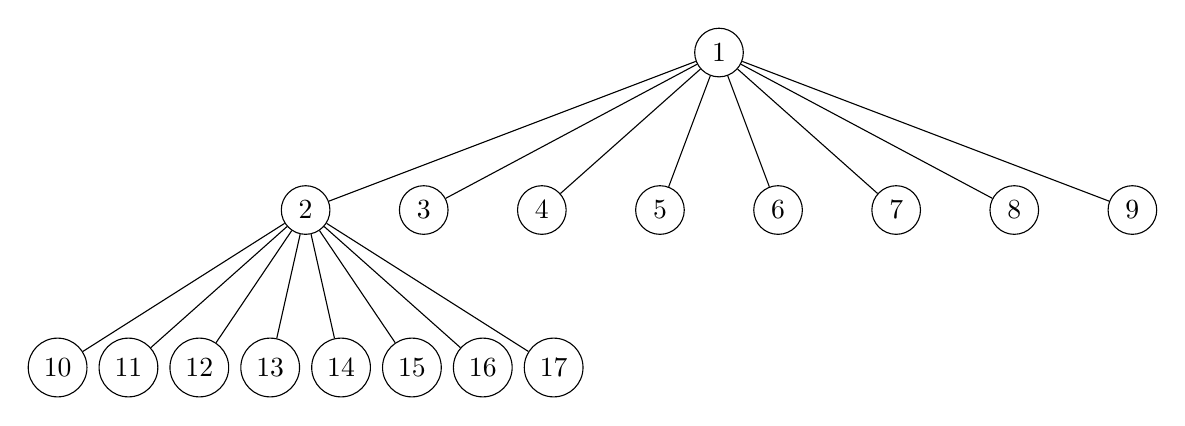
\begin{tikzpicture}
[level distance = 2cm,
level 1/.style = {sibling distance = 1.5cm},
level 2/.style = {sibling distance = 0.9cm},
]\node [draw, circle]{1}
child {node [draw, circle]{2}
child {node [draw, circle]{10}}
child {node [draw, circle]{11}}
child {node [draw, circle]{12}}
child {node [draw, circle]{13}}
child {node [draw, circle]{14}}
child {node [draw, circle]{15}}
child {node [draw, circle]{16}}
child {node [draw, circle]{17}}}
child {node [draw, circle]{3}}
child {node [draw, circle]{4}}
child {node [draw, circle]{5}}
child {node [draw, circle]{6}}
child {node [draw, circle]{7}}
child {node [draw, circle]{8}}
child {node [draw, circle]{9}};
\end{tikzpicture}
\caption{Possível árvore de suporte para a construção da fig.~\ref{fig:sierp2}.}
\label{fig:roseTreeSierp}
\end{figure}

Uma vez que o tapete é também um quadrado, o objetivo será, a partir das informações do tapete (coordenadas do vértice inferior esquerdo e comprimento do lado), desenhar o quadrado central, subdividir o tapete nos 8 sub-tapetes restantes, e voltar a desenhar, recursivamente, o quadrado nesses 8 sub-tapetes. Desta forma, cada tapete determina o seu quadrado e os seus 8 sub-tapetes. No exemplo em cima, o tapete que contém o quadrado 1 determina esse próprio quadrado e determina os sub-tapetes que contêm os quadrados 2 a 9.

Portanto, numa primeira fase, dadas as informações do tapete, é construida a árvore de suporte com todos os quadrados a desenhar, para uma determinada profundidade.
\begin{hscode}\SaveRestoreHook
\column{B}{@{}>{\hspre}l<{\hspost}@{}}%
\column{E}{@{}>{\hspre}l<{\hspost}@{}}%
\>[B]{}\Varid{squares}\mathbin{::}(\Conid{Square},\Conid{Int})\to \Conid{Rose}\;\Conid{Square}{}\<[E]%
\ColumnHook
\end{hscode}\resethooks
\ensuremath{\textbf{NB}}: No programa, a profundidade começa em $0$ e não em $1$.

Uma vez gerada a árvore com todos os quadrados a desenhar, é necessário extrair os quadrados para uma lista, a qual é processada pela função \ensuremath{\Varid{drawSq}}, disponibilizada no anexo \ref{sec:codigo}.
\begin{hscode}\SaveRestoreHook
\column{B}{@{}>{\hspre}l<{\hspost}@{}}%
\column{E}{@{}>{\hspre}l<{\hspost}@{}}%
\>[B]{}\Varid{rose2List}\mathbin{::}\Conid{Rose}\;\Varid{a}\to [\mskip1.5mu \Varid{a}\mskip1.5mu]{}\<[E]%
\ColumnHook
\end{hscode}\resethooks
Assim, a construção de tapetes de Sierpinski é dada por um hilomorfismo de \textit{Rose Trees}:
\begin{hscode}\SaveRestoreHook
\column{B}{@{}>{\hspre}l<{\hspost}@{}}%
\column{29}{@{}>{\hspre}l<{\hspost}@{}}%
\column{E}{@{}>{\hspre}l<{\hspost}@{}}%
\>[B]{}\Varid{sierpinski}\mathbin{::}(\Conid{Square},\Conid{Int})\to [\mskip1.5mu \Conid{Square}\mskip1.5mu]{}\<[E]%
\\
\>[B]{}\Varid{sierpinski}\mathrel{=}\llbracket\, \Varid{gr2l},\,{}\<[29]%
\>[29]{}\Varid{gsq}\,\rrbracket_\textit{\tiny R}{}\<[E]%
\ColumnHook
\end{hscode}\resethooks
\textbf{Trabalho a fazer:}
\begin{enumerate}
    \item Definir os genes do hilomorfismo \ensuremath{\Varid{sierpinski}}.
    \item Correr
\begin{hscode}\SaveRestoreHook
\column{B}{@{}>{\hspre}l<{\hspost}@{}}%
\column{22}{@{}>{\hspre}l<{\hspost}@{}}%
\column{E}{@{}>{\hspre}l<{\hspost}@{}}%
\>[B]{}\Varid{sierp4}\mathrel{=}\Varid{drawSq}\;(\Varid{sierpinski}\;(((\mathrm{0},\mathrm{0}),\mathrm{32}),\mathrm{3})){}\<[E]%
\\[\blanklineskip]%
\>[B]{}\Varid{constructSierp5}\mathrel{=}\mathbf{do}\;\Varid{drawSq}\;(\Varid{sierpinski}\;(((\mathrm{0},\mathrm{0}),\mathrm{32}),\mathrm{0})){}\<[E]%
\\
\>[B]{}\hsindent{22}{}\<[22]%
\>[22]{}\Varid{await}{}\<[E]%
\\
\>[B]{}\hsindent{22}{}\<[22]%
\>[22]{}\Varid{drawSq}\;(\Varid{sierpinski}\;(((\mathrm{0},\mathrm{0}),\mathrm{32}),\mathrm{1})){}\<[E]%
\\
\>[B]{}\hsindent{22}{}\<[22]%
\>[22]{}\Varid{await}{}\<[E]%
\\
\>[B]{}\hsindent{22}{}\<[22]%
\>[22]{}\Varid{drawSq}\;(\Varid{sierpinski}\;(((\mathrm{0},\mathrm{0}),\mathrm{32}),\mathrm{2})){}\<[E]%
\\
\>[B]{}\hsindent{22}{}\<[22]%
\>[22]{}\Varid{await}{}\<[E]%
\\
\>[B]{}\hsindent{22}{}\<[22]%
\>[22]{}\Varid{drawSq}\;(\Varid{sierpinski}\;(((\mathrm{0},\mathrm{0}),\mathrm{32}),\mathrm{3})){}\<[E]%
\\
\>[B]{}\hsindent{22}{}\<[22]%
\>[22]{}\Varid{await}{}\<[E]%
\\
\>[B]{}\hsindent{22}{}\<[22]%
\>[22]{}\Varid{drawSq}\;(\Varid{sierpinski}\;(((\mathrm{0},\mathrm{0}),\mathrm{32}),\mathrm{4})){}\<[E]%
\\
\>[B]{}\hsindent{22}{}\<[22]%
\>[22]{}\Varid{await}{}\<[E]%
\ColumnHook
\end{hscode}\resethooks
     \item Definir a função que apresenta a construção do tapete de Sierpinski como é apresentada em \ensuremath{\Varid{construcaoSierp5}}, mas para uma profundidade $n \in \mathbb{N}$ recebida como parâmetro.
\begin{hscode}\SaveRestoreHook
\column{B}{@{}>{\hspre}l<{\hspost}@{}}%
\column{E}{@{}>{\hspre}l<{\hspost}@{}}%
\>[B]{}\Varid{constructSierp}\mathbin{::}\Conid{Int}\to \fun{IO}\;[\mskip1.5mu ()\mskip1.5mu]{}\<[E]%
\\
\>[B]{}\Varid{constructSierp}\mathrel{=}\Varid{present}\comp \Varid{carpets}{}\<[E]%
\ColumnHook
\end{hscode}\resethooks
\textbf{Dica}: a função \ensuremath{\Varid{constructSierp}} será um hilomorfismo de listas, cujo anamorfismo \ensuremath{\Varid{carpets}\mathbin{::}\Conid{Int}\to [\mskip1.5mu [\mskip1.5mu \Conid{Square}\mskip1.5mu]\mskip1.5mu]} constrói, recebendo como parâmetro a profundidade $n$, a lista com todos os tapetes de profundidade $1..n$, e o catamorfismo \ensuremath{\Varid{present}\mathbin{::}[\mskip1.5mu [\mskip1.5mu \Conid{Square}\mskip1.5mu]\mskip1.5mu]\to \fun{IO}\;[\mskip1.5mu ()\mskip1.5mu]} percorre a lista desenhando os tapetes e esperando 1 segundo de intervalo.
\end{enumerate}

\Problema

Este ano ocorrerá a vigésima segunda edição do Campeonato do Mundo de Futebol, organizado pela Federação Internacional de Futebol (FIFA), a decorrer no Qatar e com o jogo inaugural a 20 de Novembro.

Uma casa de apostas pretende calcular, com base numa aproximação dos \textit{rankings}\footnote{Os \textit{rankings} obtidos \href{https://www.fifa.com/fifa-world-ranking/men?dateId=id13687}{aqui} foram escalados e arredondados.} das seleções, a probabilidade de cada seleção vencer a competição.

Para isso, o diretor da casa de apostas contratou o Departamento de Informática da Universidade do Minho, que atribuiu o projeto à equipa formada pelos alunos e pelos docentes de Cálculo de Programas.

\begin{alert}
Para resolver este problema de forma simples, ele será abordado por duas fases:
\begin{enumerate}
\item versão académica sem probabilidades, em que se sabe à partida, num jogo, quem o vai vencer;
\item versão realista com probabilidades usando o mónade \textit{Dist} (distribuições probabilísticas) que vem descrito no anexo \ref{sec:probabilities}.
\end{enumerate}
A primeira versão, mais simples, deverá ajudar a construir a segunda.
\end{alert}

\subsection*{Descrição do problema}

Uma vez garantida a qualificação (já ocorrida), o campeonato consta de duas fases consecutivas no tempo:
\begin{enumerate}
\item fase de grupos;
\item fase eliminatória (ou ``mata-mata'', como é habitual dizer-se no Brasil).
\end{enumerate}

Para a fase de grupos, é feito um sorteio das 32 seleções (o qual já ocorreu para esta competição)
que as coloca em 8 grupos, 4 seleções em cada grupo.
Assim, cada grupo é uma lista de seleções.

Os grupos para o campeonato deste ano são:
\begin{hscode}\SaveRestoreHook
\column{B}{@{}>{\hspre}l<{\hspost}@{}}%
\column{11}{@{}>{\hspre}l<{\hspost}@{}}%
\column{E}{@{}>{\hspre}l<{\hspost}@{}}%
\>[B]{}\mathbf{type}\;\Conid{Team}\mathrel{=}\Conid{String}{}\<[E]%
\\
\>[B]{}\mathbf{type}\;\Conid{Group}\mathrel{=}[\mskip1.5mu \Conid{Team}\mskip1.5mu]{}\<[E]%
\\[\blanklineskip]%
\>[B]{}\Varid{groups}\mathbin{::}[\mskip1.5mu \Conid{Group}\mskip1.5mu]{}\<[E]%
\\
\>[B]{}\Varid{groups}\mathrel{=}[\mskip1.5mu [\mskip1.5mu \text{\ttfamily \char34 Qatar\char34},\text{\ttfamily \char34 Ecuador\char34},\text{\ttfamily \char34 Senegal\char34},\text{\ttfamily \char34 Netherlands\char34}\mskip1.5mu],{}\<[E]%
\\
\>[B]{}\hsindent{11}{}\<[11]%
\>[11]{}[\mskip1.5mu \text{\ttfamily \char34 England\char34},\text{\ttfamily \char34 Iran\char34},\text{\ttfamily \char34 USA\char34},\text{\ttfamily \char34 Wales\char34}\mskip1.5mu],{}\<[E]%
\\
\>[B]{}\hsindent{11}{}\<[11]%
\>[11]{}[\mskip1.5mu \text{\ttfamily \char34 Argentina\char34},\text{\ttfamily \char34 Saudi~Arabia\char34},\text{\ttfamily \char34 Mexico\char34},\text{\ttfamily \char34 Poland\char34}\mskip1.5mu],{}\<[E]%
\\
\>[B]{}\hsindent{11}{}\<[11]%
\>[11]{}[\mskip1.5mu \text{\ttfamily \char34 France\char34},\text{\ttfamily \char34 Denmark\char34},\text{\ttfamily \char34 Tunisia\char34},\text{\ttfamily \char34 Australia\char34}\mskip1.5mu],{}\<[E]%
\\
\>[B]{}\hsindent{11}{}\<[11]%
\>[11]{}[\mskip1.5mu \text{\ttfamily \char34 Spain\char34},\text{\ttfamily \char34 Germany\char34},\text{\ttfamily \char34 Japan\char34},\text{\ttfamily \char34 Costa~Rica\char34}\mskip1.5mu],{}\<[E]%
\\
\>[B]{}\hsindent{11}{}\<[11]%
\>[11]{}[\mskip1.5mu \text{\ttfamily \char34 Belgium\char34},\text{\ttfamily \char34 Canada\char34},\text{\ttfamily \char34 Morocco\char34},\text{\ttfamily \char34 Croatia\char34}\mskip1.5mu],{}\<[E]%
\\
\>[B]{}\hsindent{11}{}\<[11]%
\>[11]{}[\mskip1.5mu \text{\ttfamily \char34 Brazil\char34},\text{\ttfamily \char34 Serbia\char34},\text{\ttfamily \char34 Switzerland\char34},\text{\ttfamily \char34 Cameroon\char34}\mskip1.5mu],{}\<[E]%
\\
\>[B]{}\hsindent{11}{}\<[11]%
\>[11]{}[\mskip1.5mu \text{\ttfamily \char34 Portugal\char34},\text{\ttfamily \char34 Ghana\char34},\text{\ttfamily \char34 Uruguay\char34},\text{\ttfamily \char34 Korea~Republic\char34}\mskip1.5mu]\mskip1.5mu]{}\<[E]%
\ColumnHook
\end{hscode}\resethooks
Deste modo, \textit{groups !! 0} corresponde ao grupo A, \textit{groups !! 1} ao grupo B, e assim sucessivamente.
Nesta fase, cada seleção de cada grupo vai defrontar (uma vez) as outras do seu grupo. 

Passam para o ``mata-mata'' as duas seleções que mais pontuarem em cada grupo, obtendo pontos, por cada jogo da fase grupos, da seguinte forma:
\begin{itemize}
\item vitória --- 3 pontos;
\item empate --- 1 ponto;
\item derrota --- 0 pontos.
\end{itemize}
Como se disse, a posição final no grupo irá determinar se uma seleção avança para o ``mata-mata'' e, se avançar, que possíveis jogos terá pela frente, uma vez que a disposição das seleções está desde o início definida para esta última fase, conforme se pode ver na figura \ref{fig:wcup22}.
\begin{figure}[ht]
    \centering
    \includegraphics[scale=0.125]{cp2223t_media/wcup2022.png}
    \caption{O ``mata-mata''}
    \label{fig:wcup22}
\end{figure}

Assim, é necessário calcular os vencedores dos grupos sob uma distribuição probabilística.
Uma vez calculadas as distribuições dos vencedores, é necessário colocá-las nas folhas de uma \ensuremath{{\LTree}} de forma a fazer um \textit{match} com a figura \ref{fig:wcup22}, entrando assim na fase final da competição, o tão esperado ``mata-mata''.
Para avançar nesta fase final da competição (i.e.\ subir na árvore), é preciso ganhar, quem perder é automaticamente eliminado (``mata-mata''). Quando uma seleção vence um jogo, sobe na árvore, quando perde, fica pelo caminho. Isto significa que a seleção vencedora é aquela que vence todos os jogos do ``mata-mata''.

\subsection*{Arquitetura proposta}

A visão composicional da equipa permitiu-lhe perceber desde logo que o problema podia ser dividido, independentemente da versão, probabilística ou não, em duas partes independentes --- a da fase de grupos e a do ``mata-mata''. Assim, duas sub-equipas poderiam trabalhar em paralelo, desde que se garantisse a composicionalidade das partes.
Decidiu-se que os alunos desenvolveriam a parte da fase de grupos e os docentes a do ``mata-mata''.

\subsubsection*{Versão não probabilística}
O resultado final (não probabilístico) é dado pela seguinte função:
\begin{hscode}\SaveRestoreHook
\column{B}{@{}>{\hspre}l<{\hspost}@{}}%
\column{E}{@{}>{\hspre}l<{\hspost}@{}}%
\>[B]{}\Varid{winner}\mathbin{::}\Conid{Team}{}\<[E]%
\\
\>[B]{}\Varid{winner}\mathrel{=}\Varid{wcup}\;\Varid{groups}{}\<[E]%
\\[\blanklineskip]%
\>[B]{}\Varid{wcup}\mathrel{=}\Varid{knockoutStage}\comp \Varid{groupStage}{}\<[E]%
\ColumnHook
\end{hscode}\resethooks
A sub-equipa dos docentes já entregou a sua parte:
\begin{hscode}\SaveRestoreHook
\column{B}{@{}>{\hspre}l<{\hspost}@{}}%
\column{E}{@{}>{\hspre}l<{\hspost}@{}}%
\>[B]{}\Varid{knockoutStage}\mathrel{=}\llparenthesis\, \alt{\Varid{id}}{\Varid{koCriteria}}\,\rrparenthesis{}\<[E]%
\ColumnHook
\end{hscode}\resethooks

Considere-se agora a proposta do \textit{team leader} da sub-equipa dos alunos para o desenvolvimento da fase de grupos:

\begin{bquote}
{\slshape

Vamos dividir o processo em 3 partes:
\begin{itemize}
\item gerar os jogos,
\item simular os jogos,
\item preparar o ``mata-mata'' gerando a árvore de jogos dessa fase (fig. \ref{fig:wcup22}).
\end{itemize}
Assim:
\begin{hscode}\SaveRestoreHook
\column{B}{@{}>{\hspre}l<{\hspost}@{}}%
\column{E}{@{}>{\hspre}l<{\hspost}@{}}%
\>[B]{}\Varid{groupStage}\mathbin{::}[\mskip1.5mu \Conid{Group}\mskip1.5mu]\to {\LTree}\;\Conid{Team}{}\<[E]%
\\
\>[B]{}\Varid{groupStage}\mathrel{=}\Varid{initKnockoutStage}\comp \Varid{simulateGroupStage}\comp \Varid{genGroupStageMatches}{}\<[E]%
\ColumnHook
\end{hscode}\resethooks

Comecemos então por definir a função \ensuremath{\Varid{genGroupStageMatches}} que gera os jogos da fase de grupos:
\begin{hscode}\SaveRestoreHook
\column{B}{@{}>{\hspre}l<{\hspost}@{}}%
\column{E}{@{}>{\hspre}l<{\hspost}@{}}%
\>[B]{}\Varid{genGroupStageMatches}\mathbin{::}[\mskip1.5mu \Conid{Group}\mskip1.5mu]\to [\mskip1.5mu [\mskip1.5mu \Conid{Match}\mskip1.5mu]\mskip1.5mu]{}\<[E]%
\\
\>[B]{}\Varid{genGroupStageMatches}\mathrel{=}\map \;\Varid{generateMatches}{}\<[E]%
\ColumnHook
\end{hscode}\resethooks
onde
\begin{hscode}\SaveRestoreHook
\column{B}{@{}>{\hspre}l<{\hspost}@{}}%
\column{E}{@{}>{\hspre}l<{\hspost}@{}}%
\>[B]{}\mathbf{type}\;\Conid{Match}\mathrel{=}(\Conid{Team},\Conid{Team}){}\<[E]%
\ColumnHook
\end{hscode}\resethooks
Ora, sabemos que nos foi dada a função
\begin{hscode}\SaveRestoreHook
\column{B}{@{}>{\hspre}l<{\hspost}@{}}%
\column{E}{@{}>{\hspre}l<{\hspost}@{}}%
\>[B]{}\Varid{gsCriteria}\mathbin{::}\Conid{Match}\to \Conid{Maybe}\;\Conid{Team}{}\<[E]%
\ColumnHook
\end{hscode}\resethooks
que, mediante um certo critério, calcula o resultado de um jogo, retornando \ensuremath{\Conid{Nothing}} em caso de empate, ou a equipa vencedora (sob o construtor \ensuremath{\Conid{Just}}). Assim, precisamos de definir a função
\begin{hscode}\SaveRestoreHook
\column{B}{@{}>{\hspre}l<{\hspost}@{}}%
\column{E}{@{}>{\hspre}l<{\hspost}@{}}%
\>[B]{}\Varid{simulateGroupStage}\mathbin{::}[\mskip1.5mu [\mskip1.5mu \Conid{Match}\mskip1.5mu]\mskip1.5mu]\to [\mskip1.5mu [\mskip1.5mu \Conid{Team}\mskip1.5mu]\mskip1.5mu]{}\<[E]%
\\
\>[B]{}\Varid{simulateGroupStage}\mathrel{=}\map \;(\Varid{groupWinners}\;\Varid{gsCriteria}){}\<[E]%
\ColumnHook
\end{hscode}\resethooks
que simula a fase de grupos e dá como resultado a lista dos vencedores,
recorrendo à função \ensuremath{\Varid{groupWinners}}:
\begin{hscode}\SaveRestoreHook
\column{B}{@{}>{\hspre}l<{\hspost}@{}}%
\column{E}{@{}>{\hspre}l<{\hspost}@{}}%
\>[B]{}\Varid{groupWinners}\;\Varid{criteria}\mathrel{=}\Varid{best}\;\mathrm{2}\comp \Varid{consolidate}\comp (\bind \Varid{matchResult}\;\Varid{criteria}){}\<[E]%
\ColumnHook
\end{hscode}\resethooks
Aqui está apenas em falta a definição da função \ensuremath{\Varid{matchResult}}.

Por fim, teremos a função \ensuremath{\Varid{initKnockoutStage}} que produzirá a \ensuremath{{\LTree}} que a sub-equipa do ``mata-mata'' precisa, com as devidas posições. Esta será a composição de duas funções:
\begin{hscode}\SaveRestoreHook
\column{B}{@{}>{\hspre}l<{\hspost}@{}}%
\column{E}{@{}>{\hspre}l<{\hspost}@{}}%
\>[B]{}\Varid{initKnockoutStage}\mathrel{=}\lanabracket\;\!\Varid{glt}\;\!\ranabracket\comp \Varid{arrangement}{}\<[E]%
\ColumnHook
\end{hscode}\resethooks
}
\end{bquote}
Trabalho a fazer:
\begin{enumerate}
\item	Definir uma alternativa à função genérica \ensuremath{\Varid{consolidate}} que seja um
catamorfismo de listas:
\begin{hscode}\SaveRestoreHook
\column{B}{@{}>{\hspre}l<{\hspost}@{}}%
\column{E}{@{}>{\hspre}l<{\hspost}@{}}%
\>[B]{}\Varid{consolidate'}\mathbin{::}(\Conid{Eq}\;\Varid{a},\Conid{Num}\;\Varid{b})\Rightarrow [\mskip1.5mu (\Varid{a},\Varid{b})\mskip1.5mu]\to [\mskip1.5mu (\Varid{a},\Varid{b})\mskip1.5mu]{}\<[E]%
\\
\>[B]{}\Varid{consolidate'}\mathrel{=}\llparenthesis\, \Varid{cgene}\,\rrparenthesis{}\<[E]%
\ColumnHook
\end{hscode}\resethooks
\item	Definir a função \ensuremath{\Varid{matchResult}\mathbin{::}(\Conid{Match}\to \Conid{Maybe}\;\Conid{Team})\to \Conid{Match}\to [\mskip1.5mu (\Conid{Team},\Conid{Int})\mskip1.5mu]} que apura os pontos das equipas de um dado jogo.
\item Definir a função genérica \ensuremath{\Varid{pairup}\mathbin{::}\Conid{Eq}\;\Varid{b}\Rightarrow [\mskip1.5mu \Varid{b}\mskip1.5mu]\to [\mskip1.5mu (\Varid{b},\Varid{b})\mskip1.5mu]} em que
	\ensuremath{\Varid{generateMatches}} se baseia.
\item Definir o gene \ensuremath{\Varid{glt}}.
\end{enumerate}

\subsubsection*{Versão probabilística}

Nesta versão, mais realista, \ensuremath{\Varid{gsCriteria}\mathbin{::}\Conid{Match}\to (\Conid{Maybe}\;\Conid{Team})} dá lugar a
\begin{hscode}\SaveRestoreHook
\column{B}{@{}>{\hspre}l<{\hspost}@{}}%
\column{E}{@{}>{\hspre}l<{\hspost}@{}}%
\>[B]{}\Varid{pgsCriteria}\mathbin{::}\Conid{Match}\to \fun{Dist}\;(\Conid{Maybe}\;\Conid{Team}){}\<[E]%
\ColumnHook
\end{hscode}\resethooks
que dá, para cada jogo, a probabilidade de cada equipa vencer ou haver um empate.
Por exemplo, há \ensuremath{\mathrm{50}\mathbin{\%}} de probabilidades de Portugal empatar com a Inglaterra,
\begin{quote}
\begin{tabbing}\ttfamily
~pgsCriteria\char40{}\char34{}Portugal\char34{}\char44{}\char34{}England\char34{}\char41{}\\
\ttfamily ~~~~~~~~~Nothing~~50\char46{}0\char37{}\\
\ttfamily ~~Just~\char34{}England\char34{}~~26\char46{}7\char37{}\\
\ttfamily ~Just~\char34{}Portugal\char34{}~~23\char46{}3\char37{}
\end{tabbing}
\end{quote}
etc.

O que é \ensuremath{\fun{Dist}}? É o mónade que trata de distribuições probabilísticas e que é descrito no
anexo \ref{sec:probabilities}, página \pageref{sec:probabilities} e seguintes. O que há a fazer? Eis o que diz o vosso \emph{team leader}:

\begin{bquote}
\slshape
O que há a fazer nesta versão é, antes de mais, avaliar qual é o impacto
de \ensuremath{\Varid{gsCriteria}} virar monádica (em \ensuremath{\fun{Dist}}) na arquitetura geral da versão
anterior. Há que reduzir esse impacto ao mínimo, escrevendo-se tão pouco código
quanto possível!
\end{bquote}

Todos relembraram algo que tinham aprendido nas aulas teóricas a respeito
da ``monadificação'' do código: há que reutilizar o código da versão anterior,
monadificando-o.

Para distinguir as duas versões decidiu-se afixar o prefixo `p'  para identificar
uma função que passou a ser monádica.

A sub-equipa dos docentes fez entretanto a monadificação da sua parte:
\begin{hscode}\SaveRestoreHook
\column{B}{@{}>{\hspre}l<{\hspost}@{}}%
\column{E}{@{}>{\hspre}l<{\hspost}@{}}%
\>[B]{}\Varid{pwinner}\mathbin{::}\fun{Dist}\;\Conid{Team}{}\<[E]%
\\
\>[B]{}\Varid{pwinner}\mathrel{=}\Varid{pwcup}\;\Varid{groups}{}\<[E]%
\\[\blanklineskip]%
\>[B]{}\Varid{pwcup}\mathrel{=}\Varid{pknockoutStage}\kcomp\Varid{pgroupStage}{}\<[E]%
\ColumnHook
\end{hscode}\resethooks
E entregou ainda a versão probabilística do ``mata-mata'':
\begin{hscode}\SaveRestoreHook
\column{B}{@{}>{\hspre}l<{\hspost}@{}}%
\column{9}{@{}>{\hspre}l<{\hspost}@{}}%
\column{E}{@{}>{\hspre}l<{\hspost}@{}}%
\>[B]{}\Varid{pknockoutStage}\mathrel{=}\Varid{mcataLTree'}\;\alt{\Varid{return}}{\Varid{pkoCriteria}}{}\<[E]%
\\[\blanklineskip]%
\>[B]{}\Varid{mcataLTree'}\;\Varid{g}\mathrel{=}\Varid{k}\;\mathbf{where}{}\<[E]%
\\
\>[B]{}\hsindent{9}{}\<[9]%
\>[9]{}\Varid{k}\;(\Conid{Leaf}\;\Varid{a})\mathrel{=}\Varid{g1}\;\Varid{a}{}\<[E]%
\\
\>[B]{}\hsindent{9}{}\<[9]%
\>[9]{}\Varid{k}\;(\Conid{Fork}\;(\Varid{x},\Varid{y}))\mathrel{=}\Varid{mmbin}\;\Varid{g2}\;(\Varid{k}\;\Varid{x},\Varid{k}\;\Varid{y}){}\<[E]%
\\
\>[B]{}\hsindent{9}{}\<[9]%
\>[9]{}\Varid{g1}\mathrel{=}\Varid{g}\comp i_1{}\<[E]%
\\
\>[B]{}\hsindent{9}{}\<[9]%
\>[9]{}\Varid{g2}\mathrel{=}\Varid{g}\comp i_2{}\<[E]%
\ColumnHook
\end{hscode}\resethooks
A sub-equipa dos alunos também já adiantou trabalho,
\begin{hscode}\SaveRestoreHook
\column{B}{@{}>{\hspre}l<{\hspost}@{}}%
\column{E}{@{}>{\hspre}l<{\hspost}@{}}%
\>[B]{}\Varid{pgroupStage}\mathrel{=}\Varid{pinitKnockoutStage}\kcomp\Varid{psimulateGroupStage}\comp \Varid{genGroupStageMatches}{}\<[E]%
\ColumnHook
\end{hscode}\resethooks
mas faltam ainda \ensuremath{\Varid{pinitKnockoutStage}} e \ensuremath{\Varid{pgroupWinners}}, esta usada em \ensuremath{\Varid{psimulateGroupStage}},
que é dada em anexo. 

Trabalho a fazer:
\begin{itemize}
\item	Definir as funções que ainda não estão implementadas nesta versão.
\item	\textbf{Valorização}: experimentar com outros critérios de ``ranking'' das equipas.
\end{itemize}

\begin{alert}
\textbf{Importante}: (a) código adicional terá que ser colocado no anexo
\ref{sec:resolucao}, obrigatoriamente; (b) todo o código que é dado não pode
ser alterado.
\end{alert}

\part*{Anexos}

\appendix

\section{Documentação para realizar o trabalho}
\label{sec:documentacao}
Para cumprir de forma integrada os objectivos do trabalho vamos recorrer
a uma técnica de programa\-ção dita
``\litp{literária}'' \cite{Kn92}, cujo princípio base é o seguinte:
%
\begin{quote}\em Um programa e a sua documentação devem coincidir.
\end{quote}
%
Por outras palavras, o código fonte e a documentação de um
programa deverão estar no mesmo ficheiro.

O ficheiro \texttt{cp2223t.pdf} que está a ler é já um exemplo de
\litp{programação literária}: foi gerado a partir do texto fonte
\texttt{cp2223t.lhs}\footnote{O sufixo `lhs' quer dizer
\emph{\lhaskell{literate Haskell}}.} que encontrará no
\MaterialPedagogico\ desta disciplina descompactando o ficheiro
\texttt{cp2223t.zip} e executando:
\begin{Verbatim}[fontsize=\small]
    $ lhs2TeX cp2223t.lhs > cp2223t.tex
    $ pdflatex cp2223t
\end{Verbatim}
em que \href{https://hackage.haskell.org/package/lhs2tex}{\texttt\LhsToTeX} é
um pré-processador que faz ``pretty printing''
de código Haskell em \Latex\ e que deve desde já instalar utilizando o
utiliário \href{https://www.haskell.org/cabal/}{cabal} disponível em \href{https://www.haskell.org}{haskell.org}.

Por outro lado, o mesmo ficheiro \texttt{cp2223t.lhs} é executável e contém
o ``kit'' básico, escrito em \Haskell, para realizar o trabalho. Basta executar
\begin{Verbatim}[fontsize=\small]
    $ ghci cp2223t.lhs
\end{Verbatim}

\noindent Abra o ficheiro \texttt{cp2223t.lhs} no seu editor de texto preferido
e verifique que assim é: todo o texto que se encontra dentro do ambiente
\begin{quote}\small\tt
\text{\ttfamily \char92{}begin\char123{}code\char125{}}
\\ ... \\
\text{\ttfamily \char92{}end\char123{}code\char125{}}
\end{quote}
é seleccionado pelo \GHCi\ para ser executado.

\subsection{Como realizar o trabalho}
Este trabalho teórico-prático deve ser realizado por grupos de 3 (ou 4) alunos.
Os detalhes da avaliação (datas para submissão do relatório e sua defesa
oral) são os que forem publicados na \cp{página da disciplina} na \emph{internet}.

Recomenda-se uma abordagem participativa dos membros do grupo
em todos os exercícios do trabalho, para assim
poderem responder a qualquer questão colocada na
\emph{defesa oral} do relatório.

Em que consiste, então, o \emph{relatório} a que se refere o parágrafo anterior?
É a edição do texto que está a ser lido, preenchendo o anexo \ref{sec:resolucao}
com as respostas. O relatório deverá conter ainda a identificação dos membros
do grupo de trabalho, no local respectivo da folha de rosto.

Para gerar o PDF integral do relatório deve-se ainda correr os comando seguintes,
que actualizam a bibliografia (com \Bibtex) e o índice remissivo (com \Makeindex),
\begin{Verbatim}[fontsize=\small]
    $ bibtex cp2223t.aux
    $ makeindex cp2223t.idx
\end{Verbatim}
e recompilar o texto como acima se indicou.

No anexo \ref{sec:codigo}, disponibiliza-se algum
código \Haskell\ relativo aos problemas apresentados. Esse anexo deverá
ser consultado e analisado à medida que isso for necessário.

\subsection{Como exprimir cálculos e diagramas em LaTeX/lhs2tex}
Como primeiro exemplo, estudar o texto fonte deste trabalho para obter o
efeito:\footnote{Exemplos tirados de \cite{Ol18}.}
\begin{eqnarray*}
\start
     \ensuremath{\Varid{id}\mathrel{=}\conj{\Varid{f}}{\Varid{g}}}
%
\just\equiv{ universal property }
%
        \ensuremath{\begin{lcbr}\p1\comp \Varid{id}\mathrel{=}\Varid{f}\\\p2\comp \Varid{id}\mathrel{=}\Varid{g}\end{lcbr}}
%
\just\equiv{ identity }
%
        \ensuremath{\begin{lcbr}\p1\mathrel{=}\Varid{f}\\\p2\mathrel{=}\Varid{g}\end{lcbr}}
\qed
\end{eqnarray*}

Os diagramas podem ser produzidos recorrendo à \emph{package} \LaTeX\
\href{https://ctan.org/pkg/xymatrix}{xymatrix}, por exemplo:
\begin{eqnarray*}
\xymatrix@C=2cm{
    \ensuremath{\N_0}
           \ar[d]_-{\ensuremath{\llparenthesis\, \Varid{g}\,\rrparenthesis}}
&
    \ensuremath{\mathrm{1}\mathbin{+}\N_0}
           \ar[d]^{\ensuremath{\Varid{id}\mathbin{+}\llparenthesis\, \Varid{g}\,\rrparenthesis}}
           \ar[l]_-{\ensuremath{\mathsf{in}}}
\\
     \ensuremath{\Conid{B}}
&
     \ensuremath{\mathrm{1}\mathbin{+}\Conid{B}}
           \ar[l]^-{\ensuremath{\Varid{g}}}
}
\end{eqnarray*}

\section{Regra prática para a recursividade mútua em \ensuremath{\N_0}}\label{sec:mr}

Nesta disciplina estudou-se como fazer \pd{programação dinâmica} por cálculo,
recorrendo à lei de recursividade mútua.\footnote{Lei (\ref{eq:fokkinga})
em \cite{Ol18}, página \pageref{eq:fokkinga}.}

Para o caso de funções sobre os números naturais (\ensuremath{\N_0}, com functor
\ensuremath{\fun F \;\Conid{X}\mathrel{=}\mathrm{1}\mathbin{+}\Conid{X}}) é fácil derivar-se da lei que foi estudada uma
  \emph{regra de algibeira}
  \label{pg:regra}
que se pode ensinar a programadores que não tenham estudado
\cp{Cálculo de Programas}. Apresenta-se de seguida essa regra, tomando como
exemplo o cálculo do ciclo-\textsf{for} que implementa a função de Fibonacci,
recordar o sistema:
\begin{hscode}\SaveRestoreHook
\column{B}{@{}>{\hspre}l<{\hspost}@{}}%
\column{E}{@{}>{\hspre}l<{\hspost}@{}}%
\>[B]{}\Varid{fib}\;\mathrm{0}\mathrel{=}\mathrm{1}{}\<[E]%
\\
\>[B]{}\Varid{fib}\;(\Varid{n}\mathbin{+}\mathrm{1})\mathrel{=}\Varid{f}\;\Varid{n}{}\<[E]%
\\[\blanklineskip]%
\>[B]{}\Varid{f}\;\mathrm{0}\mathrel{=}\mathrm{1}{}\<[E]%
\\
\>[B]{}\Varid{f}\;(\Varid{n}\mathbin{+}\mathrm{1})\mathrel{=}\Varid{fib}\;\Varid{n}\mathbin{+}\Varid{f}\;\Varid{n}{}\<[E]%
\ColumnHook
\end{hscode}\resethooks
Obter-se-á de imediato
\begin{hscode}\SaveRestoreHook
\column{B}{@{}>{\hspre}l<{\hspost}@{}}%
\column{4}{@{}>{\hspre}l<{\hspost}@{}}%
\column{E}{@{}>{\hspre}l<{\hspost}@{}}%
\>[B]{}\Varid{fib'}\mathrel{=}\p1\comp \for{\Varid{loop}}\ {\Varid{init}}\;\mathbf{where}{}\<[E]%
\\
\>[B]{}\hsindent{4}{}\<[4]%
\>[4]{}\Varid{loop}\;(\Varid{fib},\Varid{f})\mathrel{=}(\Varid{f},\Varid{fib}\mathbin{+}\Varid{f}){}\<[E]%
\\
\>[B]{}\hsindent{4}{}\<[4]%
\>[4]{}\Varid{init}\mathrel{=}(\mathrm{1},\mathrm{1}){}\<[E]%
\ColumnHook
\end{hscode}\resethooks
usando as regras seguintes:
\begin{itemize}
\item O corpo do ciclo \ensuremath{\Varid{loop}} terá tantos argumentos quanto o número de funções
mutuamente recursivas.
\item Para as variáveis escolhem-se os próprios nomes das funções, pela ordem
que se achar conveniente.\footnote{Podem obviamente usar-se outros símbolos,
mas numa primeira leitura dá jeito usarem-se tais nomes.}
\item Para os resultados vão-se buscar as expressões respectivas, retirando
a variável \ensuremath{\Varid{n}}.
\item Em \ensuremath{\Varid{init}} coleccionam-se os resultados dos casos de base das funções,
pela mesma ordem.
\end{itemize}
Mais um exemplo, envolvendo polinómios do segundo grau $ax^2 + b x + c$ em \ensuremath{\N_0}.
Seguindo o método estudado nas aulas\footnote{Secção 3.17 de \cite{Ol18} e tópico
\href{https://www4.di.uminho.pt/~jno/media/cp/}{Recursividade mútua}
nos vídeos de apoio às aulas teóricas.},
de $f\ x = a x^2 + b x + c$ derivam-se duas funções mutuamente recursivas:
\begin{hscode}\SaveRestoreHook
\column{B}{@{}>{\hspre}l<{\hspost}@{}}%
\column{E}{@{}>{\hspre}l<{\hspost}@{}}%
\>[B]{}\Varid{f}\;\mathrm{0}\mathrel{=}\Varid{c}{}\<[E]%
\\
\>[B]{}\Varid{f}\;(\Varid{n}\mathbin{+}\mathrm{1})\mathrel{=}\Varid{f}\;\Varid{n}\mathbin{+}\Varid{k}\;\Varid{n}{}\<[E]%
\\[\blanklineskip]%
\>[B]{}\Varid{k}\;\mathrm{0}\mathrel{=}\Varid{a}\mathbin{+}\Varid{b}{}\<[E]%
\\
\>[B]{}\Varid{k}\;(\Varid{n}\mathbin{+}\mathrm{1})\mathrel{=}\Varid{k}\;\Varid{n}\mathbin{+}\mathrm{2}\;\Varid{a}{}\<[E]%
\ColumnHook
\end{hscode}\resethooks
Seguindo a regra acima, calcula-se de imediato a seguinte implementação, em Haskell:
\begin{hscode}\SaveRestoreHook
\column{B}{@{}>{\hspre}l<{\hspost}@{}}%
\column{3}{@{}>{\hspre}l<{\hspost}@{}}%
\column{E}{@{}>{\hspre}l<{\hspost}@{}}%
\>[B]{}\Varid{f'}\;\Varid{a}\;\Varid{b}\;\Varid{c}\mathrel{=}\p1\comp \for{\Varid{loop}}\ {\Varid{init}}\;\mathbf{where}{}\<[E]%
\\
\>[B]{}\hsindent{3}{}\<[3]%
\>[3]{}\Varid{loop}\;(\Varid{f},\Varid{k})\mathrel{=}(\Varid{f}\mathbin{+}\Varid{k},\Varid{k}\mathbin{+}\mathrm{2}\mathbin{*}\Varid{a}){}\<[E]%
\\
\>[B]{}\hsindent{3}{}\<[3]%
\>[3]{}\Varid{init}\mathrel{=}(\Varid{c},\Varid{a}\mathbin{+}\Varid{b}){}\<[E]%
\ColumnHook
\end{hscode}\resethooks

\section{O mónade das distribuições probabilísticas} \label{sec:probabilities}
Mónades são functores com propriedades adicionais que nos permitem obter
efeitos especiais em progra\-mação. Por exemplo, a biblioteca \Probability\
oferece um mónade para abordar problemas de probabilidades. Nesta biblioteca,
o conceito de distribuição estatística é captado pelo tipo
\begin{eqnarray}
     \ensuremath{\mathbf{newtype}\;\fun{Dist}\;\Varid{a}\mathrel{=}\Conid{D}\;\{\mskip1.5mu \Varid{unD}\mathbin{::}[\mskip1.5mu (\Varid{a},\Conid{ProbRep})\mskip1.5mu]\mskip1.5mu\}}
     \label{eq:Dist}
\end{eqnarray}
em que \ensuremath{\Conid{ProbRep}} é um real de \ensuremath{\mathrm{0}} a \ensuremath{\mathrm{1}}, equivalente a uma escala de $0$ a
$100 \%$.

Cada par \ensuremath{(\Varid{a},\Varid{p})} numa distribuição \ensuremath{\Varid{d}\mathbin{::}\fun{Dist}\;\Varid{a}} indica que a probabilidade
de \ensuremath{\Varid{a}} é \ensuremath{\Varid{p}}, devendo ser garantida a propriedade de  que todas as probabilidades
de \ensuremath{\Varid{d}} somam $100\%$.
Por exemplo, a seguinte distribuição de classificações por escalões de $A$ a $E$,
\[
\begin{array}{ll}
A & \rule{2mm}{3pt}\ 2\%\\
B & \rule{12mm}{3pt}\ 12\%\\
C & \rule{29mm}{3pt}\ 29\%\\
D & \rule{35mm}{3pt}\ 35\%\\
E & \rule{22mm}{3pt}\ 22\%\\
\end{array}
\]
será representada pela distribuição
\begin{hscode}\SaveRestoreHook
\column{B}{@{}>{\hspre}l<{\hspost}@{}}%
\column{E}{@{}>{\hspre}l<{\hspost}@{}}%
\>[B]{}d_1 \mathbin{::}\fun{Dist}\;\Conid{Char}{}\<[E]%
\\
\>[B]{}d_1 \mathrel{=}\Conid{D}\;[\mskip1.5mu (\text{\ttfamily 'A'},\mathrm{0.02}),(\text{\ttfamily 'B'},\mathrm{0.12}),(\text{\ttfamily 'C'},\mathrm{0.29}),(\text{\ttfamily 'D'},\mathrm{0.35}),(\text{\ttfamily 'E'},\mathrm{0.22})\mskip1.5mu]{}\<[E]%
\ColumnHook
\end{hscode}\resethooks
que o \GHCi\ mostrará assim:
\begin{Verbatim}[fontsize=\small]
'D'  35.0%
'C'  29.0%
'E'  22.0%
'B'  12.0%
'A'   2.0%
\end{Verbatim}
É possível definir geradores de distribuições, por exemplo distribuições \emph{uniformes},
\begin{hscode}\SaveRestoreHook
\column{B}{@{}>{\hspre}l<{\hspost}@{}}%
\column{E}{@{}>{\hspre}l<{\hspost}@{}}%
\>[B]{}d_2 \mathrel{=}\Varid{uniform}\;(\Varid{words}\;\text{\ttfamily \char34 Uma~frase~de~cinco~palavras\char34}){}\<[E]%
\ColumnHook
\end{hscode}\resethooks
isto é
\begin{Verbatim}[fontsize=\small]
     "Uma"  20.0%
   "cinco"  20.0%
      "de"  20.0%
   "frase"  20.0%
"palavras"  20.0%
\end{Verbatim}
distribuição \emph{normais}, eg.\
\begin{hscode}\SaveRestoreHook
\column{B}{@{}>{\hspre}l<{\hspost}@{}}%
\column{E}{@{}>{\hspre}l<{\hspost}@{}}%
\>[B]{}d_3 \mathrel{=}\Varid{normal}\;[\mskip1.5mu \mathrm{10}\mathinner{\ldotp\ldotp}\mathrm{20}\mskip1.5mu]{}\<[E]%
\ColumnHook
\end{hscode}\resethooks
etc.\footnote{Para mais detalhes ver o código fonte de \Probability, que é uma adaptação da
biblioteca \PFP\ (``Probabilistic Functional Programming''). Para quem quiser saber mais
recomenda-se a leitura do artigo \cite{EK06}.}
\ensuremath{\fun{Dist}} forma um \textbf{mónade} cuja unidade é \ensuremath{\Varid{return}\;\Varid{a}\mathrel{=}\Conid{D}\;[\mskip1.5mu (\Varid{a},\mathrm{1})\mskip1.5mu]} e cuja composição de Kleisli
é (simplificando a notação)
\begin{hscode}\SaveRestoreHook
\column{B}{@{}>{\hspre}l<{\hspost}@{}}%
\column{3}{@{}>{\hspre}l<{\hspost}@{}}%
\column{E}{@{}>{\hspre}l<{\hspost}@{}}%
\>[3]{}(\Varid{f}\kcomp \Varid{g})\;\Varid{a}\mathrel{=}[\mskip1.5mu (\Varid{y},\Varid{q}\mathbin{*}\Varid{p})\mid (\Varid{x},\Varid{p})\leftarrow \Varid{g}\;\Varid{a},(\Varid{y},\Varid{q})\leftarrow \Varid{f}\;\Varid{x}\mskip1.5mu]{}\<[E]%
\ColumnHook
\end{hscode}\resethooks
em que \ensuremath{\Varid{g}\mathbin{:}\Conid{A}\to \fun{Dist}\;\mathit B} e \ensuremath{\Varid{f}\mathbin{:}\mathit B\to \fun{Dist}\;\mathit C} são funções \textbf{monádicas} que representam
\emph{computações probabilísticas}.

Este mónade é adequado à resolução de problemas de \emph{probabilidades e estatística} usando programação funcional, de forma elegante e como caso particular da programação monádica.

\section{Código fornecido}\label{sec:codigo}

\subsection*{Problema 1}
Alguns testes para se validar a solução encontrada:
\begin{hscode}\SaveRestoreHook
\column{B}{@{}>{\hspre}l<{\hspost}@{}}%
\column{E}{@{}>{\hspre}l<{\hspost}@{}}%
\>[B]{}\Varid{test}\;\Varid{a}\;\Varid{b}\;\Varid{c}\mathrel{=}\map \;(\Varid{fbl}\;\Varid{a}\;\Varid{b}\;\Varid{c})\;\Varid{x}\equiv \map \;(\Varid{f}\;\Varid{a}\;\Varid{b}\;\Varid{c})\;\Varid{x}\;\mathbf{where}\;\Varid{x}\mathrel{=}[\mskip1.5mu \mathrm{1}\mathinner{\ldotp\ldotp}\mathrm{20}\mskip1.5mu]{}\<[E]%
\\[\blanklineskip]%
\>[B]{}\Varid{test1}\mathrel{=}\Varid{test}\;\mathrm{1}\;\mathrm{2}\;\mathrm{3}{}\<[E]%
\\
\>[B]{}\Varid{test2}\mathrel{=}\Varid{test}\;(\mathbin{-}\mathrm{2})\;\mathrm{1}\;\mathrm{5}{}\<[E]%
\ColumnHook
\end{hscode}\resethooks

\subsection*{Problema 2}

\textbf{Verificação}: a árvore de tipo \Exp\ gerada por
\begin{hscode}\SaveRestoreHook
\column{B}{@{}>{\hspre}l<{\hspost}@{}}%
\column{E}{@{}>{\hspre}l<{\hspost}@{}}%
\>[B]{}\Varid{acm\char95 tree}\mathrel{=}\Varid{tax}\;\Varid{acm\char95 ccs}{}\<[E]%
\ColumnHook
\end{hscode}\resethooks
deverá verificar as propriedades seguintes:
\begin{itemize}
\item \ensuremath{\Varid{expDepth}\;\Varid{acm\char95 tree}\equiv \mathrm{7}} (profundidade da árvore);
\item \ensuremath{\length \;(\Varid{expOps}\;\Varid{acm\char95 tree})\equiv \mathrm{432}} (número de nós da árvore);
\item \ensuremath{\length \;(\Varid{expLeaves}\;\Varid{acm\char95 tree})\equiv \mathrm{1682}} (número de folhas da árvore).\footnote{Quer dizer, o número total de nodos e folhas é \ensuremath{\mathrm{2114}}, o número de linhas do texto dado.}
\end{itemize}
O resultado final
\begin{hscode}\SaveRestoreHook
\column{B}{@{}>{\hspre}l<{\hspost}@{}}%
\column{10}{@{}>{\hspre}l<{\hspost}@{}}%
\column{E}{@{}>{\hspre}l<{\hspost}@{}}%
\>[B]{}\Varid{acm\char95 xls}{}\<[10]%
\>[10]{}\mathrel{=}\Varid{post}\;\Varid{acm\char95 tree}{}\<[E]%
\ColumnHook
\end{hscode}\resethooks
não deverá ter tamanho inferior ao total de nodos e folhas da árvore.

\subsection*{Problema 3}
Função para visualização em \svg:
\begin{hscode}\SaveRestoreHook
\column{B}{@{}>{\hspre}l<{\hspost}@{}}%
\column{E}{@{}>{\hspre}l<{\hspost}@{}}%
\>[B]{}\Varid{drawSq}\;\Varid{x}\mathrel{=}\Varid{picd''}\;[\mskip1.5mu \Varid{\Conid{Svg}.scale}\;\mathrm{0.44}\;(\mathrm{0},\mathrm{0})\;(\Varid{x}\bind \Varid{sq2svg})\mskip1.5mu]{}\<[E]%
\\
\>[B]{}\Varid{sq2svg}\;(\Varid{p},\Varid{l})\mathrel{=}(\Varid{color}\;\text{\ttfamily \char34 \#67AB9F\char34}\comp \Varid{polyg})\;[\mskip1.5mu \Varid{p},\Varid{p}\mathbin{.+}(\mathrm{0},\Varid{l}),\Varid{p}\mathbin{.+}(\Varid{l},\Varid{l}),\Varid{p}\mathbin{.+}(\Varid{l},\mathrm{0})\mskip1.5mu]{}\<[E]%
\ColumnHook
\end{hscode}\resethooks
Para efeitos de temporização:
\begin{hscode}\SaveRestoreHook
\column{B}{@{}>{\hspre}l<{\hspost}@{}}%
\column{E}{@{}>{\hspre}l<{\hspost}@{}}%
\>[B]{}\Varid{await}\mathrel{=}\Varid{threadDelay}\;\mathrm{1000000}{}\<[E]%
\ColumnHook
\end{hscode}\resethooks

\subsection*{Problema 4}
Rankings:
\begin{hscode}\SaveRestoreHook
\column{B}{@{}>{\hspre}l<{\hspost}@{}}%
\column{10}{@{}>{\hspre}l<{\hspost}@{}}%
\column{E}{@{}>{\hspre}l<{\hspost}@{}}%
\>[B]{}\Varid{rankings}\mathrel{=}[\mskip1.5mu {}\<[E]%
\\
\>[B]{}\hsindent{10}{}\<[10]%
\>[10]{}(\text{\ttfamily \char34 Argentina\char34},\mathrm{4.8}),{}\<[E]%
\\
\>[B]{}\hsindent{10}{}\<[10]%
\>[10]{}(\text{\ttfamily \char34 Australia\char34},\mathrm{4.0}),{}\<[E]%
\\
\>[B]{}\hsindent{10}{}\<[10]%
\>[10]{}(\text{\ttfamily \char34 Belgium\char34},\mathrm{5.0}),{}\<[E]%
\\
\>[B]{}\hsindent{10}{}\<[10]%
\>[10]{}(\text{\ttfamily \char34 Brazil\char34},\mathrm{5.0}),{}\<[E]%
\\
\>[B]{}\hsindent{10}{}\<[10]%
\>[10]{}(\text{\ttfamily \char34 Cameroon\char34},\mathrm{4.0}),{}\<[E]%
\\
\>[B]{}\hsindent{10}{}\<[10]%
\>[10]{}(\text{\ttfamily \char34 Canada\char34},\mathrm{4.0}),{}\<[E]%
\\
\>[B]{}\hsindent{10}{}\<[10]%
\>[10]{}(\text{\ttfamily \char34 Costa~Rica\char34},\mathrm{4.1}),{}\<[E]%
\\
\>[B]{}\hsindent{10}{}\<[10]%
\>[10]{}(\text{\ttfamily \char34 Croatia\char34},\mathrm{4.4}),{}\<[E]%
\\
\>[B]{}\hsindent{10}{}\<[10]%
\>[10]{}(\text{\ttfamily \char34 Denmark\char34},\mathrm{4.5}),{}\<[E]%
\\
\>[B]{}\hsindent{10}{}\<[10]%
\>[10]{}(\text{\ttfamily \char34 Ecuador\char34},\mathrm{4.0}),{}\<[E]%
\\
\>[B]{}\hsindent{10}{}\<[10]%
\>[10]{}(\text{\ttfamily \char34 England\char34},\mathrm{4.7}),{}\<[E]%
\\
\>[B]{}\hsindent{10}{}\<[10]%
\>[10]{}(\text{\ttfamily \char34 France\char34},\mathrm{4.8}),{}\<[E]%
\\
\>[B]{}\hsindent{10}{}\<[10]%
\>[10]{}(\text{\ttfamily \char34 Germany\char34},\mathrm{4.5}),{}\<[E]%
\\
\>[B]{}\hsindent{10}{}\<[10]%
\>[10]{}(\text{\ttfamily \char34 Ghana\char34},\mathrm{3.8}),{}\<[E]%
\\
\>[B]{}\hsindent{10}{}\<[10]%
\>[10]{}(\text{\ttfamily \char34 Iran\char34},\mathrm{4.2}),{}\<[E]%
\\
\>[B]{}\hsindent{10}{}\<[10]%
\>[10]{}(\text{\ttfamily \char34 Japan\char34},\mathrm{4.2}),{}\<[E]%
\\
\>[B]{}\hsindent{10}{}\<[10]%
\>[10]{}(\text{\ttfamily \char34 Korea~Republic\char34},\mathrm{4.2}),{}\<[E]%
\\
\>[B]{}\hsindent{10}{}\<[10]%
\>[10]{}(\text{\ttfamily \char34 Mexico\char34},\mathrm{4.5}),{}\<[E]%
\\
\>[B]{}\hsindent{10}{}\<[10]%
\>[10]{}(\text{\ttfamily \char34 Morocco\char34},\mathrm{4.2}),{}\<[E]%
\\
\>[B]{}\hsindent{10}{}\<[10]%
\>[10]{}(\text{\ttfamily \char34 Netherlands\char34},\mathrm{4.6}),{}\<[E]%
\\
\>[B]{}\hsindent{10}{}\<[10]%
\>[10]{}(\text{\ttfamily \char34 Poland\char34},\mathrm{4.2}),{}\<[E]%
\\
\>[B]{}\hsindent{10}{}\<[10]%
\>[10]{}(\text{\ttfamily \char34 Portugal\char34},\mathrm{4.6}),{}\<[E]%
\\
\>[B]{}\hsindent{10}{}\<[10]%
\>[10]{}(\text{\ttfamily \char34 Qatar\char34},\mathrm{3.9}),{}\<[E]%
\\
\>[B]{}\hsindent{10}{}\<[10]%
\>[10]{}(\text{\ttfamily \char34 Saudi~Arabia\char34},\mathrm{3.9}),{}\<[E]%
\\
\>[B]{}\hsindent{10}{}\<[10]%
\>[10]{}(\text{\ttfamily \char34 Senegal\char34},\mathrm{4.3}),{}\<[E]%
\\
\>[B]{}\hsindent{10}{}\<[10]%
\>[10]{}(\text{\ttfamily \char34 Serbia\char34},\mathrm{4.2}),{}\<[E]%
\\
\>[B]{}\hsindent{10}{}\<[10]%
\>[10]{}(\text{\ttfamily \char34 Spain\char34},\mathrm{4.7}),{}\<[E]%
\\
\>[B]{}\hsindent{10}{}\<[10]%
\>[10]{}(\text{\ttfamily \char34 Switzerland\char34},\mathrm{4.4}),{}\<[E]%
\\
\>[B]{}\hsindent{10}{}\<[10]%
\>[10]{}(\text{\ttfamily \char34 Tunisia\char34},\mathrm{4.1}),{}\<[E]%
\\
\>[B]{}\hsindent{10}{}\<[10]%
\>[10]{}(\text{\ttfamily \char34 USA\char34},\mathrm{4.4}),{}\<[E]%
\\
\>[B]{}\hsindent{10}{}\<[10]%
\>[10]{}(\text{\ttfamily \char34 Uruguay\char34},\mathrm{4.5}),{}\<[E]%
\\
\>[B]{}\hsindent{10}{}\<[10]%
\>[10]{}(\text{\ttfamily \char34 Wales\char34},\mathrm{4.3})\mskip1.5mu]{}\<[E]%
\ColumnHook
\end{hscode}\resethooks
Geração dos jogos da fase de grupos:
\begin{hscode}\SaveRestoreHook
\column{B}{@{}>{\hspre}l<{\hspost}@{}}%
\column{E}{@{}>{\hspre}l<{\hspost}@{}}%
\>[B]{}\Varid{generateMatches}\mathrel{=}\Varid{pairup}{}\<[E]%
\ColumnHook
\end{hscode}\resethooks
Preparação da árvore do ``mata-mata'':
\begin{hscode}\SaveRestoreHook
\column{B}{@{}>{\hspre}l<{\hspost}@{}}%
\column{3}{@{}>{\hspre}l<{\hspost}@{}}%
\column{E}{@{}>{\hspre}l<{\hspost}@{}}%
\>[B]{}\Varid{arrangement}\mathrel{=}(\bind \Varid{swapTeams})\comp \Varid{chunksOf}\;\mathrm{4}\;\mathbf{where}{}\<[E]%
\\
\>[B]{}\hsindent{3}{}\<[3]%
\>[3]{}\Varid{swapTeams}\;[\mskip1.5mu [\mskip1.5mu a_1 ,a_2 \mskip1.5mu],[\mskip1.5mu b_1 ,b_2 \mskip1.5mu],[\mskip1.5mu c_1 ,c_2 \mskip1.5mu],[\mskip1.5mu d_1 ,d_2 \mskip1.5mu]\mskip1.5mu]\mathrel{=}[\mskip1.5mu a_1 ,b_2 ,c_1 ,d_2 ,b_1 ,a_2 ,d_1 ,c_2 \mskip1.5mu]{}\<[E]%
\ColumnHook
\end{hscode}\resethooks
Função proposta para se obter o \emph{ranking} de cada equipa:
\begin{hscode}\SaveRestoreHook
\column{B}{@{}>{\hspre}l<{\hspost}@{}}%
\column{E}{@{}>{\hspre}l<{\hspost}@{}}%
\>[B]{}\Varid{rank}\;\Varid{x}\mathrel{=}\mathrm{4}\mathbin{**}(\Varid{pap}\;\Varid{rankings}\;\Varid{x}\mathbin{-}\mathrm{3.8}){}\<[E]%
\ColumnHook
\end{hscode}\resethooks
Critério para a simulação não probabilística dos jogos da fase de grupos:
\begin{hscode}\SaveRestoreHook
\column{B}{@{}>{\hspre}l<{\hspost}@{}}%
\column{3}{@{}>{\hspre}l<{\hspost}@{}}%
\column{28}{@{}>{\hspre}l<{\hspost}@{}}%
\column{39}{@{}>{\hspre}l<{\hspost}@{}}%
\column{56}{@{}>{\hspre}l<{\hspost}@{}}%
\column{E}{@{}>{\hspre}l<{\hspost}@{}}%
\>[B]{}\Varid{gsCriteria}\mathrel{=}\Varid{s}\comp \conj{\Varid{id}\times\Varid{id}}{\Varid{rank}\times\Varid{rank}}\;\mathbf{where}{}\<[E]%
\\
\>[B]{}\hsindent{3}{}\<[3]%
\>[3]{}\Varid{s}\;((s_1 ,s_2 ),(r_1 ,r_2 ))\mathrel{=}\mathbf{let}\;\Varid{d}\mathrel{=}r_1 \mathbin{-}r_2 \;\mathbf{in}{}\<[E]%
\\
\>[3]{}\hsindent{25}{}\<[28]%
\>[28]{}\mathbf{if}\;\Varid{d}\mathbin{>}\mathrm{0.5}\;\mathbf{then}\;\Conid{Just}\;s_1 {}\<[E]%
\\
\>[28]{}\hsindent{11}{}\<[39]%
\>[39]{}\mathbf{else}\;\mathbf{if}\;\Varid{d}\mathbin{<}\mathbin{-}\mathrm{0.5}\;\mathbf{then}\;\Conid{Just}\;s_2 {}\<[E]%
\\
\>[39]{}\hsindent{17}{}\<[56]%
\>[56]{}\mathbf{else}\;\Conid{Nothing}{}\<[E]%
\ColumnHook
\end{hscode}\resethooks
Critério para a simulação não probabilística dos jogos do mata-mata:
\begin{hscode}\SaveRestoreHook
\column{B}{@{}>{\hspre}l<{\hspost}@{}}%
\column{3}{@{}>{\hspre}l<{\hspost}@{}}%
\column{28}{@{}>{\hspre}l<{\hspost}@{}}%
\column{38}{@{}>{\hspre}l<{\hspost}@{}}%
\column{E}{@{}>{\hspre}l<{\hspost}@{}}%
\>[B]{}\Varid{koCriteria}\mathrel{=}\Varid{s}\comp \conj{\Varid{id}\times\Varid{id}}{\Varid{rank}\times\Varid{rank}}\;\mathbf{where}{}\<[E]%
\\
\>[B]{}\hsindent{3}{}\<[3]%
\>[3]{}\Varid{s}\;((s_1 ,s_2 ),(r_1 ,r_2 ))\mathrel{=}\mathbf{let}\;\Varid{d}\mathrel{=}r_1 \mathbin{-}r_2 \;\mathbf{in}{}\<[E]%
\\
\>[3]{}\hsindent{25}{}\<[28]%
\>[28]{}\mathbf{if}\;\Varid{d}\equiv \mathrm{0}\;\mathbf{then}\;s_1 {}\<[E]%
\\
\>[28]{}\hsindent{10}{}\<[38]%
\>[38]{}\mathbf{else}\;\mathbf{if}\;\Varid{d}\mathbin{>}\mathrm{0}\;\mathbf{then}\;s_1 \;\mathbf{else}\;s_2 {}\<[E]%
\ColumnHook
\end{hscode}\resethooks
Critério para a simulação probabilística dos jogos da fase de grupos:
\begin{hscode}\SaveRestoreHook
\column{B}{@{}>{\hspre}l<{\hspost}@{}}%
\column{3}{@{}>{\hspre}l<{\hspost}@{}}%
\column{6}{@{}>{\hspre}l<{\hspost}@{}}%
\column{E}{@{}>{\hspre}l<{\hspost}@{}}%
\>[B]{}\Varid{pgsCriteria}\mathrel{=}\Varid{s}\comp \conj{\Varid{id}\times\Varid{id}}{\Varid{rank}\times\Varid{rank}}\;\mathbf{where}{}\<[E]%
\\
\>[B]{}\hsindent{3}{}\<[3]%
\>[3]{}\Varid{s}\;((s_1 ,s_2 ),(r_1 ,r_2 ))\mathrel{=}{}\<[E]%
\\
\>[3]{}\hsindent{3}{}\<[6]%
\>[6]{}\mathbf{if}\;\Varid{abs}\;(r_1 \mathbin{-}r_2 )\mathbin{>}\mathrm{0.5}\;\mathbf{then}\;\mathsf{fmap}\;\Conid{Just}\;(\Varid{pkoCriteria}\;(s_1 ,s_2 ))\;\mathbf{else}\;\Varid{f}\;(s_1 ,s_2 ){}\<[E]%
\\
\>[B]{}\hsindent{3}{}\<[3]%
\>[3]{}\Varid{f}\mathrel{=}\Conid{D}\comp ((\Conid{Nothing},\mathrm{0.5})\mathbin{:})\comp \map \;(\Conid{Just}\times(\mathbin{/}\mathrm{2}))\comp \Varid{unD}\comp \Varid{pkoCriteria}{}\<[E]%
\ColumnHook
\end{hscode}\resethooks
Critério para a simulação probabilística dos jogos do mata-mata:
\begin{hscode}\SaveRestoreHook
\column{B}{@{}>{\hspre}l<{\hspost}@{}}%
\column{5}{@{}>{\hspre}l<{\hspost}@{}}%
\column{E}{@{}>{\hspre}l<{\hspost}@{}}%
\>[B]{}\Varid{pkoCriteria}\;(e_1 ,e_2 )\mathrel{=}\Conid{D}\;[\mskip1.5mu (e_1 ,\mathrm{1}\mathbin{-}r_2 \mathbin{/}(r_1 \mathbin{+}r_2 )),(e_2 ,\mathrm{1}\mathbin{-}r_1 \mathbin{/}(r_1 \mathbin{+}r_2 ))\mskip1.5mu]\;\mathbf{where}{}\<[E]%
\\
\>[B]{}\hsindent{5}{}\<[5]%
\>[5]{}r_1 \mathrel{=}\Varid{rank}\;e_1 {}\<[E]%
\\
\>[B]{}\hsindent{5}{}\<[5]%
\>[5]{}r_2 \mathrel{=}\Varid{rank}\;e_2 {}\<[E]%
\ColumnHook
\end{hscode}\resethooks
Versão probabilística da simulação da fase de grupos:\footnote{Faz-se ``trimming'' das distribuições para reduzir o tempo de simulação.}
\begin{hscode}\SaveRestoreHook
\column{B}{@{}>{\hspre}l<{\hspost}@{}}%
\column{4}{@{}>{\hspre}l<{\hspost}@{}}%
\column{31}{@{}>{\hspre}l<{\hspost}@{}}%
\column{47}{@{}>{\hspre}l<{\hspost}@{}}%
\column{E}{@{}>{\hspre}l<{\hspost}@{}}%
\>[B]{}\Varid{psimulateGroupStage}\mathrel{=}\Varid{trim}\comp {}\<[31]%
\>[31]{}\map \;(\Varid{pgroupWinners}\;\Varid{pgsCriteria}){}\<[E]%
\\
\>[B]{}\Varid{trim}\mathrel{=}\Varid{top}\;\mathrm{5}\comp \Varid{sequence}\comp \map \;(\Varid{filterP}\comp \Varid{norm})\;{}\<[47]%
\>[47]{}\mathbf{where}{}\<[E]%
\\
\>[B]{}\hsindent{4}{}\<[4]%
\>[4]{}\Varid{filterP}\;(\Conid{D}\;\Varid{x})\mathrel{=}\Conid{D}\;[\mskip1.5mu (\Varid{a},\Varid{p})\mid (\Varid{a},\Varid{p})\leftarrow \Varid{x},\Varid{p}\mathbin{>}\mathrm{0.0001}\mskip1.5mu]{}\<[E]%
\\
\>[B]{}\hsindent{4}{}\<[4]%
\>[4]{}\Varid{top}\;\Varid{n}\mathrel{=}\Varid{vec2Dist}\comp \Varid{take}\;\Varid{n}\comp \Varid{reverse}\comp \Varid{presort}\;\p2\comp \Varid{unD}{}\<[E]%
\\
\>[B]{}\hsindent{4}{}\<[4]%
\>[4]{}\Varid{vec2Dist}\;\Varid{x}\mathrel{=}\Conid{D}\;[\mskip1.5mu (\Varid{a},\Varid{n}\mathbin{/}\Varid{t})\mid (\Varid{a},\Varid{n})\leftarrow \Varid{x}\mskip1.5mu]\;\mathbf{where}\;\Varid{t}\mathrel{=}\Varid{sum}\;(\map \;\p2\;\Varid{x}){}\<[E]%
\ColumnHook
\end{hscode}\resethooks
Versão mais eficiente da \ensuremath{\Varid{pwinner}} dada no texto principal, para diminuir o tempo de cada
simulação:
\begin{hscode}\SaveRestoreHook
\column{B}{@{}>{\hspre}l<{\hspost}@{}}%
\column{4}{@{}>{\hspre}l<{\hspost}@{}}%
\column{E}{@{}>{\hspre}l<{\hspost}@{}}%
\>[B]{}\Varid{pwinner}\mathbin{::}\fun{Dist}\;\Conid{Team}{}\<[E]%
\\
\>[B]{}\Varid{pwinner}\mathrel{=}\Varid{mbin}\;\Varid{f}\;\Varid{x}\bind \Varid{pknockoutStage}\;\mathbf{where}{}\<[E]%
\\
\>[B]{}\hsindent{4}{}\<[4]%
\>[4]{}\Varid{f}\;(\Varid{x},\Varid{y})\mathrel{=}\Varid{initKnockoutStage}\;(\Varid{x}\mathbin{+\!\!\!+}\Varid{y}){}\<[E]%
\\
\>[B]{}\hsindent{4}{}\<[4]%
\>[4]{}\Varid{x}\mathrel{=}\conj{\Varid{g}\comp \Varid{take}\;\mathrm{4}}{\Varid{g}\comp \Varid{drop}\;\mathrm{4}}\;\Varid{groups}{}\<[E]%
\\
\>[B]{}\hsindent{4}{}\<[4]%
\>[4]{}\Varid{g}\mathrel{=}\Varid{psimulateGroupStage}\comp \Varid{genGroupStageMatches}{}\<[E]%
\ColumnHook
\end{hscode}\resethooks
Auxiliares:
\begin{hscode}\SaveRestoreHook
\column{B}{@{}>{\hspre}l<{\hspost}@{}}%
\column{E}{@{}>{\hspre}l<{\hspost}@{}}%
\>[B]{}\Varid{best}\;\Varid{n}\mathrel{=}\map \;\p1\comp \Varid{take}\;\Varid{n}\comp \Varid{reverse}\comp \Varid{presort}\;\p2{}\<[E]%
\\[\blanklineskip]%
\>[B]{}\Varid{consolidate}\mathbin{::}(\Conid{Num}\;\Varid{d},\Conid{Eq}\;\Varid{d},\Conid{Eq}\;\Varid{b})\Rightarrow [\mskip1.5mu (\Varid{b},\Varid{d})\mskip1.5mu]\to [\mskip1.5mu (\Varid{b},\Varid{d})\mskip1.5mu]{}\<[E]%
\\
\>[B]{}\Varid{consolidate}\mathrel{=}\map \;(\Varid{id}\times\Varid{sum})\comp \Varid{collect}{}\<[E]%
\\[\blanklineskip]%
\>[B]{}\Varid{collect}\mathbin{::}(\Conid{Eq}\;\Varid{a},\Conid{Eq}\;\Varid{b})\Rightarrow [\mskip1.5mu (\Varid{a},\Varid{b})\mskip1.5mu]\to [\mskip1.5mu (\Varid{a},[\mskip1.5mu \Varid{b}\mskip1.5mu])\mskip1.5mu]{}\<[E]%
\\
\>[B]{}\Varid{collect}\;\Varid{x}\mathrel{=}\Varid{nub}\;[\mskip1.5mu \Varid{k}\mapsto[\mskip1.5mu \Varid{d'}\mid (\Varid{k'},\Varid{d'})\leftarrow \Varid{x},\Varid{k'}\equiv \Varid{k}\mskip1.5mu]\mid (\Varid{k},\Varid{d})\leftarrow \Varid{x}\mskip1.5mu]{}\<[E]%
\ColumnHook
\end{hscode}\resethooks
Função binária monádica \ensuremath{\Varid{f}}:
\begin{hscode}\SaveRestoreHook
\column{B}{@{}>{\hspre}l<{\hspost}@{}}%
\column{E}{@{}>{\hspre}l<{\hspost}@{}}%
\>[B]{}\Varid{mmbin}\mathbin{::}\Conid{Monad}\;\Varid{m}\Rightarrow ((\Varid{a},\Varid{b})\to \Varid{m}\;\Varid{c})\to (\Varid{m}\;\Varid{a},\Varid{m}\;\Varid{b})\to \Varid{m}\;\Varid{c}{}\<[E]%
\\
\>[B]{}\Varid{mmbin}\;\Varid{f}\;(\Varid{a},\Varid{b})\mathrel{=}\mathbf{do}\;\{\mskip1.5mu \Varid{x}\leftarrow \Varid{a};\Varid{y}\leftarrow \Varid{b};\Varid{f}\;(\Varid{x},\Varid{y})\mskip1.5mu\}{}\<[E]%
\ColumnHook
\end{hscode}\resethooks
Monadificação de uma função binária \ensuremath{\Varid{f}}:
\begin{hscode}\SaveRestoreHook
\column{B}{@{}>{\hspre}l<{\hspost}@{}}%
\column{E}{@{}>{\hspre}l<{\hspost}@{}}%
\>[B]{}\Varid{mbin}\mathbin{::}\Conid{Monad}\;\Varid{m}\Rightarrow ((\Varid{a},\Varid{b})\to \Varid{c})\to (\Varid{m}\;\Varid{a},\Varid{m}\;\Varid{b})\to \Varid{m}\;\Varid{c}{}\<[E]%
\\
\>[B]{}\Varid{mbin}\mathrel{=}\Varid{mmbin}\comp (\Varid{return}\comp ){}\<[E]%
\ColumnHook
\end{hscode}\resethooks
Outras funções que podem ser úteis:
\begin{hscode}\SaveRestoreHook
\column{B}{@{}>{\hspre}l<{\hspost}@{}}%
\column{E}{@{}>{\hspre}l<{\hspost}@{}}%
\>[B]{}(\Varid{f}\mathbin{`\Varid{is}`}\Varid{v})\;\Varid{x}\mathrel{=}(\Varid{f}\;\Varid{x})\equiv \Varid{v}{}\<[E]%
\\[\blanklineskip]%
\>[B]{}\Varid{rcons}\;(\Varid{x},\Varid{a})\mathrel{=}\Varid{x}\mathbin{+\!\!\!+}[\mskip1.5mu \Varid{a}\mskip1.5mu]{}\<[E]%
\ColumnHook
\end{hscode}\resethooks

%----------------- Soluções dos alunos -----------------------------------------%

\section{Soluções dos alunos}\label{sec:resolucao}
Os alunos devem colocar neste anexo as suas soluções para os exercícios
propostos, de acordo com o ``layout'' que se fornece. Não podem ser
alterados os nomes ou tipos das funções dadas, mas pode ser adicionado
texto, diagramas e/ou outras funções auxiliares que sejam necessárias.

Valoriza-se a escrita de \emph{pouco} código que corresponda a soluções
simples e elegantes.

\subsection*{Problema 1}
Funções auxiliares pedidas:
\begin{hscode}\SaveRestoreHook
\column{B}{@{}>{\hspre}l<{\hspost}@{}}%
\column{E}{@{}>{\hspre}l<{\hspost}@{}}%
\>[B]{}\Varid{loop}\;\Varid{a}\;\Varid{b}\;\Varid{c}\mathrel{=}\Varid{fblLoop}\;\Varid{a}\;\Varid{b}\;\Varid{c}{}\<[E]%
\\
\>[B]{}\Varid{initial}\mathrel{=}((\mathrm{0},\mathrm{0}),\mathrm{0}){}\<[E]%
\\
\>[B]{}\Varid{wrap}\mathrel{=}\p2{}\<[E]%
\ColumnHook
\end{hscode}\resethooks

\subsubsection{Primeira tentativa}

Numa primeira abordagem a este problema, tentamos reduzir analiticamente 
a função dada, f, de maneira a que o seu nível de operação passasse de (n+3) 
para (n+1). Contudo, após algumas tentativas, não conseguimos deduzir as dependências 
que se traduziam nas funções mútuamente recursivas. Apesar disso, conseguimos 
perceber que há um pormenor que se manteve nesta tentativa de solução, o facto de haver 
necessidade de construir esta nova função através de três funções, tal como já nos 
sugeria a original ao ser constituída por três casos base, na sua definição (não é uma regra, mas 
pode induzir para o resultado correto).\\

\subsubsection{Segunda tentativa}

Numa fase em que a solução não estava a ser muito fácil de calcular, tentamos seguir rumo pelo 
desenho de diagramas e uma pré-configuração de como o sistema se deveria comportar.
Para tal, configuramos o seguinte diagrama para nos auxiliar neste processo.

\begin{eqnarray*}
\xymatrix@C=3cm{
    N \ar[d]_{<<h,g>,f>} \ar@/^/[r]^{out Nat_0} & 1 + N \ar[d]^{F<<h,g>, f>} \ar@/^/[l]^{in Nat_0} \\
     (A\times B)\times C & F((A \times B) \times C) \ar[l]^{<<k,j>,i>}
}
\end{eqnarray*}

Como estamos a operar sobre números naturais, N, sabemos como se comportam os in e out dos mesmos.

\begin{lstlisting}
in = [0, succ]
out 0 = Left ()
out (n+1) = Right n
\end{lstlisting}

Já que não conseguimos deduzir diretamente as funções necessárias, podemos atentar em como o sistema 
se deverá comportar para, desde o início, chegar à solução, recursivamente. Ora, preparando um 
esquema com dados relativos às respetivas soluções, chegamos ao seguinte:

\begin{lstlisting}
                   c=1  b=1  a=1
N = 0    Left ()    ((_, _), 0)
N = 1    Right 0    ((_, _), 1)
N = 2    Right 1    ((_, _), 1)
N = 3    Right 2    ((_, _), 2)
N = 4    Right 3    ((_, _), 4)
N = 5    Right 4    ((_, _), 7)
N = 6    Right 5    ((_, _), 13)
N = 7    Right 6    ((_, _), 24)

                   c=3  b=2  a=1
N = 0    Left ()    ((_, _), 0)
N = 1    Right 0    ((_, _), 1)
N = 2    Right 1    ((_, _), 1)
N = 3    Right 2    ((_, _), 3)
N = 4    Right 3    ((_, _), 8)
N = 5    Right 4    ((_, _), 17)
N = 6    Right 5    ((_, _), 42)
N = 7    Right 6    ((_, _), 100)

\end{lstlisting}

A partir de um dado inteiro, conseguimos deduzir como as funções mutuamente recursivas se devem comportar.\\
Ora, o resultado já nos é apresentado pelo enunciado do problema, sendo colocado no último elemento da 
nossa configuração pela prestação definida da função \textbf{warp=p2}, cujo objetivo é retirar o resultado do problema.\\
Os inteiros e a sua configuração do \textbf{out} servem meramente como guias para nos orientarmos no processo de recursividade.\\
Passando para os primeiros três resultados, apesar dos diferentes fatores 'a', 'b' e 'c', percebemos que estes são 
constantes, o que faz sentido de acordo com a definição original da função f.
Assim, basta-nos encontrar relações entre os valores, com o auxílio desses fatores, que, a partir de um nível anterior, consigam 
definir o resultado do nível seguinte.

Após um curto período de experimentação, chegamos às seguintes relações:

\begin{enumerate}

  \item O primeiro elemento de um nível é o segundo do nível anterior.
  \item O segundo elemento é o terceiro do nível anterior.
  \item O terceiro elemento é o somatório de cada um dos elementos do nível anterior, multiplicado pelo seu fator.

\end{enumerate}

Seguindo as regras apresentadas acima, chegamos à seguinte configuração (para os espaços em falta, sugere-se a aplicação 
das referidas regras, de maneira a perceber o processo intrínseco à configuração):

\begin{lstlisting}
                   c=1  b=1  a=1
N = 0    Left ()    ((0, 0), 0)
N = 1    Right 0    ((0, 0), 1)
N = 2    Right 1    ((0, 1), 1)
N = 3    Right 2    ((1, 1), 2)
N = 4    Right 3    ((1, 2), 4)
N = 5    Right 4    ((2, 4), 7)
N = 6    Right 5    ((_, _), 13)
N = 7    Right 6    ((_, _), 24)

                   c=3  b=2  a=1
N = 0    Left ()    ((_, _), 0)
N = 1    Right 0    ((_, _), 1)
N = 2    Right 1    ((_, _), 1)
N = 3    Right 2    ((_, 1), 3)
N = 4    Right 3    ((1, 3), 8)
N = 5    Right 4    ((3, 8), 17)
N = 6    Right 5    ((8, 17), 42)
N = 7    Right 6    ((17, 42), 100)

\end{lstlisting}

Traduzindo as relações identificadas, chegamos à seguinte configuração:

\begin{hscode}\SaveRestoreHook
\column{B}{@{}>{\hspre}l<{\hspost}@{}}%
\column{E}{@{}>{\hspre}l<{\hspost}@{}}%
\>[B]{}\mbox{\onelinecomment  initial = ((0, 0), 0)\\}{}\<[E]%
\\[\blanklineskip]%
\>[B]{}\mbox{\onelinecomment  fblH a b c ((ee, ed), d) = ed}{}\<[E]%
\\
\>[B]{}\Varid{fblH}\;\Varid{a}\;\Varid{b}\;\Varid{c}\mathrel{=}\p2\comp \p1{}\<[E]%
\\[\blanklineskip]%
\>[B]{}\mbox{\onelinecomment  \\}{}\<[E]%
\\
\>[B]{}\mbox{\onelinecomment  fblG a b c ((ee, ed), d) = d}{}\<[E]%
\\
\>[B]{}\Varid{fblG}\;\Varid{a}\;\Varid{b}\;\Varid{c}\mathrel{=}\p2{}\<[E]%
\\[\blanklineskip]%
\>[B]{}\mbox{\onelinecomment  \\}{}\<[E]%
\\
\>[B]{}\mbox{\onelinecomment  fblF a b c ((ee, ed), d) = a * d + b * ed + c * ee}{}\<[E]%
\\
\>[B]{}\Varid{fblF}\;\anonymous \;\anonymous \;\anonymous \;((\anonymous ,\anonymous ),\mathrm{0})\mathrel{=}\mathrm{1}{}\<[E]%
\\
\>[B]{}\Varid{fblF}\;\anonymous \;\anonymous \;\anonymous \;((\anonymous ,\mathrm{0}),\mathrm{1})\mathrel{=}\mathrm{1}{}\<[E]%
\\
\>[B]{}\Varid{fblF}\;\Varid{a}\;\Varid{b}\;\Varid{c}\;((\Varid{ee},\Varid{ed}),\Varid{d})\mathrel{=}\Varid{a}\mathbin{*}\Varid{d}\mathbin{+}\Varid{b}\mathbin{*}\Varid{ed}\mathbin{+}\Varid{c}\mathbin{*}\Varid{ee}{}\<[E]%
\\[\blanklineskip]%
\>[B]{}\mbox{\onelinecomment  \\}{}\<[E]%
\\
\>[B]{}\mbox{\onelinecomment  \textless h, g \textgreater = \textless fblH, fblG \textgreater}{}\<[E]%
\\
\>[B]{}\Varid{fblHG}\;\Varid{a}\;\Varid{b}\;\Varid{c}\mathrel{=}\conj{\Varid{fblH}\;\Varid{a}\;\Varid{b}\;\Varid{c}}{\Varid{fblG}\;\Varid{a}\;\Varid{b}\;\Varid{c}}{}\<[E]%
\\[\blanklineskip]%
\>[B]{}\mbox{\onelinecomment  \\}{}\<[E]%
\\
\>[B]{}\mbox{\onelinecomment  \textless \textless h, g \textgreater , f \textgreater = \textless fblHG, fblF \textgreater}{}\<[E]%
\\
\>[B]{}\Varid{fblLoop}\;\Varid{a}\;\Varid{b}\;\Varid{c}\mathrel{=}\conj{\Varid{fblHG}\;\Varid{a}\;\Varid{b}\;\Varid{c}}{\Varid{fblF}\;\Varid{a}\;\Varid{b}\;\Varid{c}}{}\<[E]%
\ColumnHook
\end{hscode}\resethooks


De maneira a justificar a necessidade de evoluir certos algoritmos para a sua versão em recursividade mútua, fizemos alguns testes com ambas 
as versões desta função, f e fbl. Para recolher as métricas utilizamos o comando ":set +s" para ativar as estatísticas de tempo e espaço, das quais 
conseguimos retirar informações como o tempo gasto pelo CPU e o número de \textit{bytes} da memória necessários para executar os cálculos necessários.
Na primeira tabela, as reticências devem-se a um tempo de espera tão demorado que não conseguimos obter os resultados. Na segunda, o único valor com o 
mesmo formato deve-se a ser um número tão grande que não se encaixa no formato da tabela.\\

\begin{center}
\begin{tabular}{|c c c c c c c c|} 
 \hline
 Function & a & b & c & n & CPU Time (secs) & \#Bytes of memory & Answer \\ [0.5ex] 
 \hline\hline
 f & 1 & 2 & 3 & 5 & 0,00 & 63,840 & 17 \\ 
 \hline
 f & 1 & 2 & 3 & 10 & 0,01 & 214,504 & 1331 \\
 \hline
 f & 1 & 2 & 3 & 15 & 0,02 & 3,356,080 & 100425 \\
 \hline
 f & 1 & 2 & 3 & 20 & 0,27 & 69,456,856 & 7579198\\
 \hline
 f & 1 & 2 & 3 & 25 & 5,91 & 1,460,849,568 & 572024206 \\ 
 \hline
 f & 1 & 2 & 3 & 30 & 132.30 & 30,749,309,288 & 43172337417 \\ 
 \hline
  f & 1 & 2 & 3 & 35 & ... & ... & ... \\ 
 \hline
\end{tabular}
\end{center}

\begin{center}
\begin{tabular}{|c c c c c c c c|} 
 \hline
 Function & a & b & c & n & CPU Time (secs) & \#Bytes of memory & Answer \\ [0.5ex] 
 \hline\hline
 fbl & 1 & 2 & 3 & 5 & 0,00 & 66,496 & 17 \\ 
 \hline
 fbl & 1 & 2 & 3 & 10 & 0,00 & 76,632 & 1331 \\
 \hline
 fbl & 1 & 2 & 3 & 15 & 0,00 & 86,768 & 100425 \\
 \hline
 fbl & 1 & 2 & 3 & 20 & 0,01 & 96,216 & 7579198\\
 \hline
 fbl & 1 & 2 & 3 & 25 & 0,01 & 106,352 & 572024206 \\ 
 \hline
 fbl & 1 & 2 & 3 & 30 & 0,01 & 116,488 & 43172337417 \\ 
 \hline
 fbl & 1 & 2 & 3 & 100 & 0,01 & 266,768 & 8,4E+36 \\ 
 \hline
 fbl & 1 & 2 & 3 & 1000 & 0,03 &  2,721,432 & ... \\ 
 \hline
\end{tabular}
\end{center}


\subsection*{Problema 2}
Gene de \ensuremath{\Varid{tax}}:
\begin{hscode}\SaveRestoreHook
\column{B}{@{}>{\hspre}l<{\hspost}@{}}%
\column{E}{@{}>{\hspre}l<{\hspost}@{}}%
\>[B]{}\Varid{gene}\mathrel{=}\Varid{ggene}{}\<[E]%
\ColumnHook
\end{hscode}\resethooks

\subsubsection{Primeiro passo: hierarquias}

O problema é-nos apresentado, desde logo, como contendo um tipo de hierarquia entre os seus elementos, 
sendo os mesmos \textit{strings}. A hierarquia é definida pelo número de espaços em braco que contém no 
seu início, até alcançar um caracter diferente. A cada quatro espaços brancos, incrementa-se um nível.

\begin{lstlisting}
    #espacos    #hierarquia    
        0            0
        4            1
        8            2
      (...)        (...)
\end{lstlisting}

A partir daqui, podemos, desde já, definir as funções que arrecadarão com o trabalho de retirar o nível de 
hierarquia de cada uma das \textit{strings}.

\begin{hscode}\SaveRestoreHook
\column{B}{@{}>{\hspre}l<{\hspost}@{}}%
\column{3}{@{}>{\hspre}l<{\hspost}@{}}%
\column{E}{@{}>{\hspre}l<{\hspost}@{}}%
\>[B]{}\mbox{\onelinecomment  calculate the number of 'space' characters in the beginning of the string\\}{}\<[E]%
\\
\>[B]{}\Varid{initialSpaces}\;(\Varid{h}\mathbin{:}\Varid{t}){}\<[E]%
\\
\>[B]{}\hsindent{3}{}\<[3]%
\>[3]{}\mid \Varid{h}\equiv \text{\ttfamily '~'}\mathrel{=}\succ \;(\Varid{initialSpaces}\;\Varid{t}){}\<[E]%
\\
\>[B]{}\hsindent{3}{}\<[3]%
\>[3]{}\mid \Varid{otherwise}\mathrel{=}\mathrm{0}{}\<[E]%
\\[\blanklineskip]%
\>[B]{}\mbox{\onelinecomment  calculate the hierarchy level of current string\\}{}\<[E]%
\\
\>[B]{}\Varid{expHierarchyLevel}\;\Varid{str}\mathrel{=}\Varid{n\char95 spaces}\div \mathrm{4}{}\<[E]%
\\
\>[B]{}\hsindent{3}{}\<[3]%
\>[3]{}\mathbf{where}\;\Varid{n\char95 spaces}\mathrel{=}\Varid{initialSpaces}\;\Varid{str}{}\<[E]%
\ColumnHook
\end{hscode}\resethooks

\subsubsection{Segundo passo: gene do anamorfismo}

O diagrama apresentado no enunciado já nos mostra como parte do gene deste anamorfismo se comporta.
Ao utilizar o out de listas não vazias, ou temos um único elemento, ou a cabeça da lista e a cauda da mesma, como na 
configuração do out aplicado a listas normais.

\begin{eqnarray*}
\xymatrix@C=2cm{
    S^* \ar[r]^{out} & \textcolor{orange}{S + S} \times \textcolor{blue}{S^*} \ar[r]^{...} & \textcolor{orange}{S + S} \times \textcolor{blue}{(S^*)^*}
}
\end{eqnarray*}

A partir da linha acima exposta, percebemos que, quando aplicado, o nosso gene tem de preparar os valores 
que recebe com o formato correto para que o bifuntor de base opere na recursividade. Assim, a partir de 
(\textit{S + S}) temos de transformar no tipo (\textit{S + S}), enquanto no lado de \textit{S*} precisamos transformar 
esta lista numa lista de listas, \textit{(S*)*}.\\

Tratando-se de uma disjunção, o nosso gene será obrigatoriamente do tipo (algo + algo).\\
Sendo uma execução em paralelo, do lado direito, o gene será, por sua vez, do tipo (algo + (algo \times algo)).\\

Caso tenhamos um único elemento, o construtor de \textit{Exp Tree} consegue lidar com ele, há apenas necessidade 
de o preservar (identidade). O mesmo acontece para a cabeça de uma lista. Esta será um nodo pai na consequente árvore, 
restando apenas definir os seus filhos (identidade).\\
Ora, a partir disto, conseguimos definir algo como sendo do tipo (id + (id \times algo)).\\

Como o objetivo é pegar numa lista e transformá-la numa lista de listas, temos já uma dica de que é necessário agrupar 
valores. A questão é: Como? Com que restrições/fatores? Ora, temos a indicação de que temos de seguir uma determinada 
hierarquia e o cálculo da mesma já está preparado (primeiro passo). Assim, apenas precisamos de encontrar uma função que 
agrupe elementos tendo em conta uma determinada relação entre eles, algo que já existe: \textit{groupBy}.\\

Desta maneira, agrupamos elementos de uma lista cujo nível hierárquico esteja em ordem crescente de valores!

\begin{hscode}\SaveRestoreHook
\column{B}{@{}>{\hspre}l<{\hspost}@{}}%
\column{E}{@{}>{\hspre}l<{\hspost}@{}}%
\>[B]{}\mbox{\onelinecomment  after the out of a non-empty list, this is the gene\\}{}\<[E]%
\\
\>[B]{}\Varid{ggene}\mathrel{=}(\Varid{id}+(\Varid{id}\times\Varid{groupBy}\;(\lambda \Varid{x}\;\Varid{y}\to \Varid{expHierarchyLevel}\;\Varid{x}\mathbin{<}\Varid{expHierarchyLevel}\;\Varid{y})))\comp \Varid{out}{}\<[E]%
\ColumnHook
\end{hscode}\resethooks


Função de pós-processamento:
\begin{hscode}\SaveRestoreHook
\column{B}{@{}>{\hspre}l<{\hspost}@{}}%
\column{E}{@{}>{\hspre}l<{\hspost}@{}}%
\>[B]{}\Varid{post}\mathbin{::}\Conid{Exp}\;\Conid{String}\;\Conid{String}\to [\mskip1.5mu [\mskip1.5mu \Conid{String}\mskip1.5mu]\mskip1.5mu]{}\<[E]%
\\
\>[B]{}\Varid{post}\;(\Conid{Var}\;\Varid{s})\mathrel{=}[\mskip1.5mu [\mskip1.5mu \Varid{s}\mskip1.5mu]\mskip1.5mu]{}\<[E]%
\\
\>[B]{}\Varid{post}\;(\Conid{Term}\;\Varid{a}\;[\mskip1.5mu \mskip1.5mu])\mathrel{=}[\mskip1.5mu [\mskip1.5mu \Varid{a}\mskip1.5mu]\mskip1.5mu]{}\<[E]%
\\
\>[B]{}\Varid{post}\;(\Conid{Term}\;\Varid{s}\;\Varid{es})\mathrel{=}[\mskip1.5mu [\mskip1.5mu \Varid{s}\mskip1.5mu]\mskip1.5mu]\mathbin{+\!\!\!+}\map \;(\Varid{s}\mathbin{:})\;(\Varid{concatMap}\;\Varid{post}\;\Varid{es}){}\<[E]%
\ColumnHook
\end{hscode}\resethooks

\subsection*{Problema 3}
\begin{hscode}\SaveRestoreHook
\column{B}{@{}>{\hspre}l<{\hspost}@{}}%
\column{E}{@{}>{\hspre}l<{\hspost}@{}}%
\>[B]{}\Varid{squares}\mathrel{=}\lanabracket\;\!\Varid{gsq}\;\!\ranabracket_\textit{\tiny R}{}\<[E]%
\\
\>[B]{}\Varid{gsq}\mathrel{=}\Varid{divide\char95 }{}\<[E]%
\\
\>[B]{}\Varid{rose2List}\mathrel{=}\llparenthesis\, \Varid{gr2l}\,\rrparenthesis_\textit{\tiny R}{}\<[E]%
\\
\>[B]{}\Varid{gr2l}\mathrel{=}(\Varid{cons}\comp (\Varid{id}\times\Varid{concat})){}\<[E]%
\\
\>[B]{}\Varid{carpets}\mathrel{=}\Varid{reverse}\comp \anaList{\Varid{carpets\char95 gene}}{}\<[E]%
\\[\blanklineskip]%
\>[B]{}\Varid{present}\mathbin{::}[\mskip1.5mu [\mskip1.5mu \Conid{Square}\mskip1.5mu]\mskip1.5mu]\to \fun{IO}\;[\mskip1.5mu ()\mskip1.5mu]{}\<[E]%
\\
\>[B]{}\Varid{present}\mathrel{=}\llparenthesis\, \Varid{ppresent}\,\rrparenthesis{}\<[E]%
\ColumnHook
\end{hscode}\resethooks

\subsubsection{Primeiro passo - anamorfismo de Rose Tree}

Um hilomorfismo é constituído por um catamorfismo após um anamorfismo. Nesta sequência, precisamos preliminarmente de 
definir o anamorfismo que construirá uma \textit{Rose tree} a partir do \textit{input} que a função 
\textit{squares} recebe: \textit{(Square, Int)}.\\

Ora, traduzindo o tipo de entrada para um tipo mais genérico, podemos ter o seguinte:\\

  \textcolor{blue}{Square} = ((x, y), side) = ((A \times B) \times C)\\
  (Square, \textcolor{orange}{Int}) = \textcolor{blue}{((A \times B) \times C)} \textcolor{orange} { \times P }
\\

Sobre \textit{rose trees} sabemos ainda que:

\begin{eqnarray*}
\xymatrix@C=3cm{
    Rose\ A \ar@/^1pc/[r]^{out} & A \times (Rose\ A)^* \ar@/^1pc/[l]^{in}
}
\end{eqnarray*}

Assim, podemos preparar já o diagrama que define o anamorfismo a construir.

\begin{eqnarray*}
\xymatrix@C=3cm{
    (((A \times B) \times C) \times P) \ar[d]^{[(divide)]} \ar[r]^{divide} & ((A \times B) \times C) \times (((A \times B) \times C) \times P) \ar[d]^{B(id, 
\ [(divide)])}\\
    Rose ((A \times B) \times C) \ar@/^1pc/[r]^{out} & ((A \times B) \times C) \times Rose ((A \times B) \times C)^* \ar@/^1pc/[l]^{in}
}
\end{eqnarray*}

Com o diagrama feito, basta preparar os pontos. Para cada ponto de referência, temos de calcular os oito pontos 
relativos. Tivemos cuidado para ordenar esses pontos consoante a ordem relativa esquerda-direita, baixo-cima para produzir 
o efeito da ordem utilizada nas figuras fornecidas no enunciado do problema.\\
Calculados os pontos, o anamorfismo faz todo o trabalho restante por nós, pegando nos pontos que criamos e transformando-os 
na respetiva \textit{rose tree}.

\begin{hscode}\SaveRestoreHook
\column{B}{@{}>{\hspre}l<{\hspost}@{}}%
\column{3}{@{}>{\hspre}l<{\hspost}@{}}%
\column{E}{@{}>{\hspre}l<{\hspost}@{}}%
\>[B]{}\Varid{divide\char95 }\;((((\Varid{x},\Varid{y}),\Varid{l}),\mathrm{0}))\mathrel{=}((((\Varid{x}\mathbin{+}(\Varid{l}\mathbin{/}\mathrm{3}),\Varid{y}\mathbin{+}(\Varid{l}\mathbin{/}\mathrm{3})),\Varid{l}\mathbin{/}\mathrm{3}),[\mskip1.5mu \mskip1.5mu])){}\<[E]%
\\
\>[B]{}\Varid{divide\char95 }\;((((\Varid{x},\Varid{y}),\Varid{l}),\Varid{p}))\mathrel{=}((((\Varid{x}\mathbin{+}\Varid{sndLvl},\Varid{y}\mathbin{+}\Varid{sndLvl}),\Varid{sndLvl}),\Varid{x1}\mathbin{+\!\!\!+}\Varid{x2}\mathbin{+\!\!\!+}\Varid{x3})){}\<[E]%
\\
\>[B]{}\hsindent{3}{}\<[3]%
\>[3]{}\mathbf{where}{}\<[E]%
\\
\>[B]{}\hsindent{3}{}\<[3]%
\>[3]{}\Varid{sndLvl}\mathrel{=}(\Varid{l}\mathbin{/}\mathrm{3}){}\<[E]%
\\
\>[B]{}\hsindent{3}{}\<[3]%
\>[3]{}\Varid{thdLvl}\mathrel{=}\Varid{sndLvl}\mathbin{*}\mathrm{2}{}\<[E]%
\\
\>[B]{}\hsindent{3}{}\<[3]%
\>[3]{}\Varid{newP}\mathrel{=}\Varid{p}\mathbin{-}\mathrm{1}{}\<[E]%
\\
\>[B]{}\hsindent{3}{}\<[3]%
\>[3]{}\Varid{x1}\mathrel{=}(((\Varid{x},\Varid{y}\mathbin{+}\Varid{thdLvl}),\Varid{sndLvl}),\Varid{newP})\mathbin{:}(((\Varid{x}\mathbin{+}\Varid{sndLvl},\Varid{y}\mathbin{+}\Varid{thdLvl}),\Varid{sndLvl}),\Varid{newP})\mathbin{:}(((\Varid{x}\mathbin{+}\Varid{thdLvl},\Varid{y}\mathbin{+}\Varid{thdLvl}),\Varid{sndLvl}),\Varid{newP})\mathbin{:}[\mskip1.5mu \mskip1.5mu]{}\<[E]%
\\
\>[B]{}\hsindent{3}{}\<[3]%
\>[3]{}\Varid{x2}\mathrel{=}(((\Varid{x},\Varid{y}\mathbin{+}\Varid{sndLvl}),\Varid{sndLvl}),\Varid{newP})\mathbin{:}(((\Varid{x}\mathbin{+}\Varid{thdLvl},\Varid{y}\mathbin{+}\Varid{sndLvl}),\Varid{sndLvl}),\Varid{newP})\mathbin{:}[\mskip1.5mu \mskip1.5mu]{}\<[E]%
\\
\>[B]{}\hsindent{3}{}\<[3]%
\>[3]{}\Varid{x3}\mathrel{=}(((\Varid{x},\Varid{y}),\Varid{sndLvl}),\Varid{newP})\mathbin{:}(((\Varid{x}\mathbin{+}\Varid{sndLvl},\Varid{y}),\Varid{sndLvl}),\Varid{newP})\mathbin{:}(((\Varid{x}\mathbin{+}\Varid{thdLvl},\Varid{y}),\Varid{sndLvl}),\Varid{newP})\mathbin{:}[\mskip1.5mu \mskip1.5mu]{}\<[E]%
\ColumnHook
\end{hscode}\resethooks

\subsubsection{Segundo passo - catamorfismo}

O trabalho do catamorfismo \textit{rose2List} é, como o nome indica, transformar uma \textit{Rose tree} numa lista, 
contendo esta os quadrados a desenhar que se encontravam na árvore.\\

Partindo, novamente, de um diagrama, temos:

\begin{eqnarray*}
\xymatrix@C=2cm{
    Rose ((A \times B) \times C) \ar[d]_{(|gr2l|)} \ar@/^1pc/[r]^{outRose} & ((A \times B) \times C) \times (Rose (A \times B) \times C)^* \ar[d]^{id + (|gr2l|)} \ar@/^1pc/[l]^{inRose}\\
    ((A \times B) \times C)^* & ((A \times B) \times C) \times Rose ((A \times B) \times C)^* \ar@/2pc/[l]^{g=[\_, \_]}
}
\end{eqnarray*}

Para formar uma lista a partir de uma cabeça e o resto do seu corpo, basta utilizarmos a função \textit{cons}.
Contudo, como temos listas de listas, temos de reduzir a complexidade desse tipo para apenas uma lista, logo:

\begin{lstlisting}
  g = cons . (id x concat)
\end{lstlisting}

Aqui, temos a construção de uma lista após preservar a sua cabeça e reduzir a complexidade da sua cauda.


\subsubsection{Terceiro Passo - anamorfismo \textit{carpets}}

Mais uma vez, é-nos pedida a construção de um hilomorfismo (catamorfismo após anamorfismo), desta vez para automatizar o precesso 
de construção dos gráficos com os quadrados de \textit{Sierpisnki}.\\
Ora, o anamorfismo \textit{carpets} recebe um inteiro e produz uma lista com listas de quadrados que definem cada um dos níveis de 
profundidade do tapete. Assim, conseguimos reproduzir o seguinte diagrama:

\begin{eqnarray*}
\xymatrix@C=2cm{
    N \ar[r]^{outNat} \ar[d]_{[(carpets)]} & 1 + N \ar@/-3pc/[r]^{id + <N,N>} & 1 + ((A \times B) \times C)^* \times ((A \times B) \times C)^* \ar[d]^{id+id\times[(carpets)]}\\
(((A \times B) \times C)^*)^* && 1 + ((A \times B) \times C)^* \times (((A \times B) \times C)^*)^* \ar@/5pc/[ll]_{inList}
}
\end{eqnarray*}

Queremos, portanto, a partir de um número, criar recursivamente as listas que irão definir os \textit{squares} de cada nível de 
profundidade do carpete. Como já temos uma função que faz esse trabalho, \textit{Sierpinski}, basta atribuir-lhe um valor arbitrário:

\begin{hscode}\SaveRestoreHook
\column{B}{@{}>{\hspre}l<{\hspost}@{}}%
\column{E}{@{}>{\hspre}l<{\hspost}@{}}%
\>[B]{}\mbox{\onelinecomment  then, we can use it as pointfree\\}{}\<[E]%
\\
\>[B]{}\Varid{draw32}\;\Varid{n}\mathrel{=}\Varid{sierpinski}\;(((\mathrm{0},\mathrm{0}),\mathrm{32}),\Varid{n}){}\<[E]%
\\
\>[B]{}\Varid{carpets\char95 gene}\mathrel{=}(\Varid{id}+\conj{\Varid{draw32}}{\Varid{id}})\comp \Varid{outNat}{}\<[E]%
\ColumnHook
\end{hscode}\resethooks

Aqui, não fazemos nada no nível de profundidade zero (preservar com identidade). Contudo, a partir de um inteiro natural processamos 
a respetiva lista de \textit{squares} associado a esse nível e preservamos o mesmo valor para a próxima iteração da recursividade o voltar 
a processar. No fim, o construtor de listas será capaz de transformar este trabalho numa única lista com os tapetes de cada nível de 
profundidade.\\

\subsubsection{Quarto passo - catamorfismo \textit{present}}

O catamorfimos final deve processar a lista de tapetes criada anteriormente e, percorrendo cada tapete, deve desenhá-lo, respeitando um 
intervalo de um segundo entre cada gráfico gerado.\\
Assumindo que nunca vamos ter uma lista sem pontos (i.e., usamos um catamorfismo de listas não vazias), o gene deste catamorfismo tem de ser capaz de lidar com dois casos: quando a lista tem 
um único tapete, ou quando tem um tapete à cabeça de uma lista e os restantes tapetes na cauda da mesma. Tratando-se de uma disjunção, 
definimos dois casos para um gene \textit{ppresent} que se limita a utilizar a função fornecida para desenho de carpetes:


\begin{hscode}\SaveRestoreHook
\column{B}{@{}>{\hspre}l<{\hspost}@{}}%
\column{E}{@{}>{\hspre}l<{\hspost}@{}}%
\>[B]{}\Varid{ppresent}\;(i_1\;\Varid{a})\mathrel{=}\mathbf{do}\;\Varid{drawSq}\;\Varid{a};\Varid{await};\Varid{return}\;[\mskip1.5mu \mskip1.5mu]{}\<[E]%
\\
\>[B]{}\Varid{ppresent}\;(i_2\;(\Varid{h},\Varid{t}))\mathrel{=}\mathbf{do}\;\Varid{drawSq}\;\Varid{h};\Varid{await};\mathbf{do}\;\Varid{t}{}\<[E]%
\ColumnHook
\end{hscode}\resethooks

\subsection*{Problema 4}
\subsubsection*{Versão não probabilística}
Gene de \ensuremath{\Varid{consolidate'}}:

\begin{hscode}\SaveRestoreHook
\column{B}{@{}>{\hspre}l<{\hspost}@{}}%
\column{E}{@{}>{\hspre}l<{\hspost}@{}}%
\>[B]{}\Varid{cgene}\mathbin{::}(\Conid{Eq}\;\Varid{a},\Conid{Num}\;\Varid{b})\Rightarrow \Varid{c}+((\Varid{a},\Varid{b}),[\mskip1.5mu (\Varid{a},\Varid{b})\mskip1.5mu])\to [\mskip1.5mu (\Varid{a},\Varid{b})\mskip1.5mu]{}\<[E]%
\\
\>[B]{}\Varid{cgene}\mathrel{=}\alt{\Varid{nil}}{\Varid{pairConsolidate2}}{}\<[E]%
\\[\blanklineskip]%
\>[B]{}\Varid{pairConsolidate2}\;(\Varid{a},[\mskip1.5mu \mskip1.5mu])\mathrel{=}\Varid{singl}\;\Varid{a}{}\<[E]%
\\
\>[B]{}\Varid{pairConsolidate2}\;((\Varid{a},\Varid{b}),((\Varid{h1},\Varid{h2})\mathbin{:}\Varid{t})){}\<[E]%
\\
\>[B]{}\mid \Varid{a}\equiv \Varid{h1}\mathrel{=}(\Varid{h1},\Varid{h2}\mathbin{+}\Varid{b})\mathbin{:}\Varid{t}{}\<[E]%
\\
\>[B]{}\mid \Varid{otherwise}\mathrel{=}(\Varid{h1},\Varid{h2})\mathbin{:}\Varid{pairConsolidate2}\;((\Varid{a},\Varid{b}),\Varid{t}){}\<[E]%
\ColumnHook
\end{hscode}\resethooks

Para calcular o gene para o catamorfismo de listas pedido, consolidate', limitamo-nos a construir uma função que fosse 
capaz de lidar com o tipo gerado pelo \textit{out} das listas. Assim, como caso de paragem assumimos ter um único elemento do lado 
esquerdo e vazio no direito e, nos restantes, vamos percorrendo a lista do lado direito até encontrar valores cujas condições se apliquem 
ao caso de utilização do \textit{consolidate}.


Geração dos jogos da fase de grupos:
\begin{hscode}\SaveRestoreHook
\column{B}{@{}>{\hspre}l<{\hspost}@{}}%
\column{3}{@{}>{\hspre}l<{\hspost}@{}}%
\column{E}{@{}>{\hspre}l<{\hspost}@{}}%
\>[B]{}\Varid{pairup}\mathrel{=}\Varid{concat}\comp \anaList{\Varid{pairupGene}}{}\<[E]%
\\
\>[B]{}\Varid{pairupGene}\mathrel{=}(\Varid{id}+\conj{\Varid{pairupEsq}}{\p2})\comp \Varid{outList}{}\<[E]%
\\[\blanklineskip]%
\>[B]{}\Varid{pairupEsq}\;(\Varid{team},[\mskip1.5mu \mskip1.5mu])\mathrel{=}[\mskip1.5mu \mskip1.5mu]{}\<[E]%
\\
\>[B]{}\Varid{pairupEsq}\;(\Varid{team},\Varid{h}\mathbin{:}[\mskip1.5mu \mskip1.5mu])\mathrel{=}[\mskip1.5mu (\Varid{team},\Varid{h})\mskip1.5mu]{}\<[E]%
\\
\>[B]{}\Varid{pairupEsq}\;(\Varid{team},\Varid{h}\mathbin{:}\Varid{t})\mathrel{=}(\Varid{team},\Varid{h})\mathbin{:}\Varid{pairupEsq}\;(\Varid{team},\Varid{t}){}\<[E]%
\\[\blanklineskip]%
\>[B]{}\Varid{matchResult}\mathbin{::}(\Conid{Match}\to \Conid{Maybe}\;\Conid{Team})\to \Conid{Match}\to [\mskip1.5mu (\Conid{Team},\Conid{Int})\mskip1.5mu]{}\<[E]%
\\
\>[B]{}\Varid{matchResult}\;\Varid{criteria}\;(\Varid{m1},\Varid{m2})\mathrel{=}[\mskip1.5mu (\Varid{m1},r_1 ),(\Varid{m2},r_2 )\mskip1.5mu]\;\mathbf{where}{}\<[E]%
\\
\>[B]{}\hsindent{3}{}\<[3]%
\>[3]{}\Varid{winner}\mathrel{=}\Varid{criteria}\;(\Varid{m1},\Varid{m2}){}\<[E]%
\\
\>[B]{}\hsindent{3}{}\<[3]%
\>[3]{}r_1 \mathrel{=}\mathbf{if}\;\Varid{winner}\equiv \Conid{Nothing}\;\mathbf{then}\;\mathrm{0}\;\mathbf{else}\;\mathbf{if}\;\Varid{winner}\equiv \Conid{Just}\;\Varid{m1}\;\mathbf{then}\;\mathrm{3}\;\mathbf{else}\;\mathrm{1}{}\<[E]%
\\
\>[B]{}\hsindent{3}{}\<[3]%
\>[3]{}r_2 \mathrel{=}\mathbf{if}\;r_1 \equiv \mathrm{0}\;\mathbf{then}\;\mathrm{0}\;\mathbf{else}\;\mathbf{if}\;r_1 \equiv \mathrm{3}\;\mathbf{then}\;\mathrm{1}\;\mathbf{else}\;\mathrm{3}{}\<[E]%
\\[\blanklineskip]%
\>[B]{}\Varid{glt}\mathrel{=}(\Varid{id}+(\Varid{singl}\times\Varid{id}))\comp \Varid{out}{}\<[E]%
\ColumnHook
\end{hscode}\resethooks

Para definir \textit{pairup}, consideramos que este é um anamorfismo que pega 
numa lista de equipas e a transforma numa lista de pares contendo todos os \textit{matches} 
possíveis dentro de um determinado grupo. Como o resultado obtido é uma lista com listas, 
aplicas o \textit{concat} para as reduzir a uma única lista, como pretendido.

\begin{eqnarray*}
\xymatrix@C=3cm{
    T^* \ar[r]^{outList} \ar[d]_{f} & 1 + T \times T^* \ar@/-1pc/[r]^{id + <pairupEsq, \pi2>} & 1 + (T \times T)^* \times (T)^* 
 \ar[d]^{id + id \times f^*}\\
((T \times T)^*)^* && 1 + (T \times T)^* \times (T \times T)^* \ar@/5pc/[ll]_{inList}
}
\end{eqnarray*}


\subsubsection*{Versão probabilística}
\begin{hscode}\SaveRestoreHook
\column{B}{@{}>{\hspre}l<{\hspost}@{}}%
\column{E}{@{}>{\hspre}l<{\hspost}@{}}%
\>[B]{}\Varid{pinitKnockoutStage}\mathrel{=}\bot {}\<[E]%
\\[\blanklineskip]%
\>[B]{}\Varid{pgroupWinners}\mathbin{::}(\Conid{Match}\to \fun{Dist}\;(\Conid{Maybe}\;\Conid{Team}))\to [\mskip1.5mu \Conid{Match}\mskip1.5mu]\to \fun{Dist}\;[\mskip1.5mu \Conid{Team}\mskip1.5mu]{}\<[E]%
\\
\>[B]{}\Varid{pgroupWinners}\mathrel{=}\bot {}\<[E]%
\\[\blanklineskip]%
\>[B]{}\Varid{pmatchResult}\mathrel{=}\bot {}\<[E]%
\ColumnHook
\end{hscode}\resethooks

%----------------- Índice remissivo (exige makeindex) -------------------------%

\printindex

%----------------- Bibliografia (exige bibtex) --------------------------------%

\bibliographystyle{plain}
\bibliography{cp2223t}

%----------------- Fim do documento -------------------------------------------%

\end{document}
